
\newif\ifsubmit
%\submitfalse
\submittrue           % uncomment this line for submission.


\newcount\usepng\usepng=1               % use PNG versions of figures (smaller file)


\documentclass[manuscript, screen, anonymous=false]{acmart}

%% Rights management information.  This information is sent to you
%% when you complete the rights form.  These commands have SAMPLE
%% values in them; it is your responsibility as an author to replace
%% the commands and values with those provided to you when you
%% complete the rights form.
\setcopyright{acmcopyright}
\copyrightyear{2023}
\acmYear{2023}
\acmDOI{XXXXXXX.XXXXXXX}

%% These commands are for a JOURNAL article.
\acmJournal{TECS}
\acmVolume{0}
\acmNumber{0}
\acmArticle{111}
\acmMonth{6}

\usepackage{balance} % For balanced columns on the last page
\usepackage[normalem]{ulem}


\usepackage{graphicx}  % for \includegraphics


\ifsubmit
\usepackage[final]{fixme}
\else
\usepackage[draft]{fixme}
\fxsetup{
    author=,
    layout=inline,
    theme=colorsig
}
\fi
\newcommand{\xxx}{\fxwarning}


\usepackage{url}
\def\UrlBreaks{\do\/\do-}


\usepackage{siunitx}
%\usepackage{SIunits}


\ifnum\usepng=1
 \DeclareGraphicsExtensions{.png,.eps,.ps,.jpg}
\else
 \DeclareGraphicsExtensions{.ps,.eps,.png,.jpg}
\fi

\usepackage{ifpdf}
\ifpdf
\setlength{\pdfpagewidth}{8.5in}
\setlength{\pdfpageheight}{11in}
\else
\fi

\usepackage{microtype}
\usepackage{paralist}

%stuff for better looking tables
\usepackage{array}
\usepackage{booktabs}
\usepackage{multirow}
\usepackage{dcolumn}
\pdfcompresslevel=9       % highly compressed pdf

\newlength{\thinline}
\setlength{\thinline}{0.05em}
\newlength{\thickline}
\setlength{\thickline}{0.10em}
\newcommand{\ra}[1]{\renewcommand{\arraystretch}{#1}}
\newcolumntype{.}{D{.}{.}{-1}}

\usepackage{enumitem} % to fiddle with enumerate spacing

\usepackage{subcaption}
\usepackage{xspace}
% pretty captions: small text, bold figure title
%\usepackage[bf]{caption}
%\DeclareCaptionType{copyrightbox}
%\renewcommand{\captionfont}{\normalsize}


\newcommand{\headingg}[1]{\textbf{#1}}
\newcommand{\term}[1]{\emph{#1}}
\newcommand{\nowrapterm}[1]{\mbox{\emph{#1}}}
\newcommand{\secref}[1]{\mbox{Section~\ref{#1}}}
\newcommand{\plursecref}[1]{\mbox{Sections~{#1}}}
\newcommand{\symsecref}[1]{\mbox{\S~\ref{#1}}}
\newcommand{\plursymsecref}[1]{\mbox{\S\S~{#1}}}
\newcommand{\figref}[1]{\mbox{Figure~\ref{#1}}}
\newcommand{\tabref}[1]{\mbox{Table~\ref{#1}}}
\newcommand{\tblref}[1]{\tabref{#1}}
\newcommand{\algref}[1]{\mbox{Algorithm~\ref{#1}}}
\newcommand{\listingref}[1]{\mbox{Listing~\ref{#1}}}

% textual substitutions
\newcommand{\etal}{\mbox{et al.}}
\newcommand{\ie}{\textit{i.e.,}}
\newcommand{\eg}{\textit{e.g.,}}

%\newcommand{\degree}{\ensuremath{^\circ}}
\newcommand{\iv}{I--\kern-.08emV\xspace}

% No-indent paragraphs
\newcommand{\noind}[0]{\vspace{5 pt} \noindent}
\newcommand{\noindpar}[1]{\noind {\bf #1}}
%\newcommand{\noindpar}[1]{\noind \textbf{\small{#1}}}

\newcommand{\textoverline}[1]{$\overline{\mbox{#1}}$}

% Macros for notes, comments, and todo.
\ifsubmit
  \newcommand{\colorcomment}[3]{\relax}
  \newcommand{\greencomment}[2]{\relax}
  \newcommand{\yellowcomment}[2]{\relax}
  \newcommand{\cyancomment}[2]{\relax}
  \newcommand{\bluecomment}[2]{\relax}
  \newcommand{\redcomment}[2]{\relax}
  \newcommand{\magentacomment}[2]{\relax}

  \newcommand{\hey}[1]{\relax}
  \newcommand{\bibtex}[1]{\relax}
  \newcommand{\task}[1]{\relax}
  \newcommand{\question}[1]{\relax}
  \newcommand{\note}[1]{\relax}

\else
  % comment commands
  % comments should be signed at the end with the initials of the comment writer.
  \newcommand{\colorcomment}[3]{\par\noindent\textcolor{#1}{[{#2}: {#3}]}\par} % general case
  \newcommand{\greencomment}[2]{\colorcomment{green}{#1}{#2}} % hard to read
  \newcommand{\yellowcomment}[2]{\colorcomment{yellow}{#1}{#2}} % hard to read
  \newcommand{\cyancomment}[2]{\colorcomment{cyan}{#1}{#2}} % hard to read
  \newcommand{\bluecomment}[2]{\colorcomment{blue}{#1}{#2}}
  \newcommand{\redcomment}[2]{\colorcomment{red}{#1}{#2}}
  \newcommand{\magentacomment}[2]{\colorcomment{magenta}{#1}{#2}}

  \newcommand{\hey}[1]{\textcolor{magenta}{[{#1}]}} % quick inline comment
  \newcommand{\note}[1]{\magentacomment{Note}{#1}} % a paragraph comment.
  \newcommand{\bibtex}[1]{\magentacomment{@bibtex}{#1}} % a reference that should go to bibtex
  \newcommand{\task}[1]{\redcomment{Task}{#1}} % task the person with @name in the argument
  \newcommand{\question}[1]{\bluecomment{Q?}{#1}} % ask a question
\fi

\usepackage{listings}
\usepackage{color}

\definecolor{mygreen}{rgb}{0,0.6,0}
\definecolor{mygray}{rgb}{0.5,0.5,0.5}
\definecolor{mymauve}{rgb}{0.58,0,0.82}
\definecolor{myred}{rgb}{0.58,0,0.0}
\lstset{
    language=C,
         emph={when},
         basicstyle=\footnotesize\ttfamily,
         numberstyle=\tiny,
         numbersep=5pt,
         tabsize=2,
         extendedchars=true,
         breaklines=true,
                keywordstyle=\color{mymauve}\ttfamily\bfseries,
                emphstyle=\color{mymauve}\ttfamily\bfseries,
                stringstyle=\color{myred}\ttfamily,
                commentstyle=\color{mygreen}\ttfamily,
                morecomment=[l][\color{mygray}]{\#},
         showspaces=false,
         showtabs=false,
         %xleftmargin=17pt,
         %framexleftmargin=17pt,
         %framexrightmargin=5pt,
         framexbottommargin=4pt,
         escapeinside={\%*}{*)},
         showstringspaces=false
 }

%\usepackage{caption}
%\DeclareCaptionFont{white}{\color{white}}
%\DeclareCaptionFormat{listing}{\colorbox[cmyk]{0.43, 0.35, 0.35,0.01}{\parbox{\columnwidth}{\hspace{15pt}#1#2#3}}}
%\captionsetup[lstlisting]{format=listing,labelfont=white,textfont=white, singlelinecheck=false, margin=0pt, font={bf,footnotesize}}

%\setcopyright{acmcopyright} % if you give the rights to ACM
%\acmDOI{...} % DOI - Insert your DOI below...
%\acmISBN{...} % ISBN - Insert your conference/workshop's ISBN below...
%\acmYear{2023} % Insert Publication year
%\copyrightyear{2023} % Insert Copyright year (typically the same as above)
%\acmPrice{15.00}
%\acmConference[SenSys]{The 17th ACM Conference on Embedded Network Sensor Systems}{November 10-13, 2019}
%{New York, New York, USA}
%\acmJournal{TOSN}

\hyphenation{WISP RFID CRFID CRFIDs RF volt-age}
\newcommand{\sysnameraw}{Waldo}
\newcommand{\sysname}{\sysnameraw\xspace}
\newcommand{\sysnames}{\sysnameraw{}s\xspace}
\newcommand{\numExp}{881\xspace} %updated by Nicole 1/30
\newcommand{\numDet}{881\xspace}
\newcommand{\numDir}{849\xspace} %updated by Nicole 1/30
\newcommand{\numDoors}{7\xspace}  %updated by Nicole 1/25
\newcommand{\numPeople}{9\xspace}  %updated by Nicole 1/25 - need to double check this
\newcommand{\SysAccuracy}{100\%\xspace} %updated by Nicole 1/25
\newcommand{\dirAccuracy}{96.4\%\xspace} %updated by Nicole 1/25
\newcommand{\minSeparation}{3-4 seconds\xspace}
\newcommand{\ITWdays}{64 days\xspace}
\newcommand{\ITWdeployedWaldos}{5\xspace}
\newcommand{\ITWpeopleEvents}{xxx\xspace}
\newcommand{\WaldoPWR}{wwPWR\xspace}
\newcommand{\EnoceanPWR}{eeePWR\xspace}


\usepackage{pifont}% http://ctan.org/pkg/pifont
\newcommand{\cmark}{\ding{51}}%
\newcommand{\xmark}{\ding{55}}%
%\newcommand{\syslongname}{\textbf{W}aldo, \textbf{A} \textbf{L}ow-power \textbf{D}oorjamb \textbf{O}ccupancy-tracker\xspace}
%\newcommand{\sysname}{LumiJamb\xspace}
%\newcommand{\syslongname}{\textbf{Lumi}nance based people tracking in the Door\textbf{Jamb}\xspace}
%\newcommand{\sysname}{SolarJamb\xspace}
%\newcommand{\syslongname}{\textbf{Solar} based people tracking in the Door\textbf{Jamb}\xspace}

\begin{document}
%\nocaptionrule % This removes the ugly line above table captions on SIGPLAN templates

\clubpenalty=10000
\widowpenalty=10000

\title[Batteryless Occupancy Monitoring with \sysname]{\sysname: Batteryless Occupancy Monitoring using Reflected Ambient Light}
%\title[Doorway Sensing with \sysname]{Batteryless Occupancy Monitoring with Reflected Ambient Light}
%Alternative Title suggestion:  "Waldo: An Unobtrusive Batteryless Doorway Sensor for Room-Level Occupancy Tracking using Reflected Ambient Light". -NT


\author{Nicole Tobias}  %ORCID: 0000-0003-4895-6792
\affiliation{%
  \institution{Clemson University}
  \city{Clemson}
  \country{USA}
  }
\email{rtobias@clemson.edu}

\author{Harsh Desai}  %ORCID:
\affiliation{%
  \institution{Carnegie Mellon University}
  \city{Pittsburgh}
  \country{USA}
  }
\email{harshd@andrew.cmu.edu}

\author{Arwa Alsubhi}  %ORCID: 0000-0003-3912-8143
\affiliation{%
  \institution{Clemson University}
  \city{Clemson}
  \country{USA}
  }
\email{aalsubh@clemson.edu}

\author{Calvin Moody}  %ORCID:
\affiliation{%
  \institution{Facet Wealth}
  \city{Baltimore}
  \country{USA}
  }
%\email{cmmoody@clemson.edu}
\email{calvinmcm@gmail.com}

\author{Josiah Hester}  %ORCID:
\affiliation{%
  \institution{Georgia Institute of Technology}
  \city{Atlanta}
  \country{USA}
  }
\email{josiah@gatech.edu}

\author{Jacob Sorber}  %ORCID: 
\affiliation{%
  \institution{Clemson University}
  \city{Clemson}
  \country{USA}
  }
\email{jsorber@clemson.edu}

\renewcommand{\shortauthors}{N. Tobias et al.}


\begin{abstract}
The buildings of our science fiction dreams have always adapted to the needs of their occupants.
Today, "smart buildings" are poised to become reality, enabled by advances in sensors that monitor room-level occupancy and movement.
Unfortunately, existing occupancy-tracking systems are plagued by large size, high energy consumption, and, unsurprisingly, short battery lifetimes.

In this paper, we present \sysname, a \textit{batteryless}, room-level occupancy monitoring sensor that harvests energy from indoor ambient light reflections, and uses changes in these reflections to detect when people enter and exit a room.
%This information is then communicated by radio to a basestation for further processing and actuation.
Like previous systems, \sysname is mountable at the top of a doorframe, allowing for detection and tracking of a person at the entry and exit point of a room.
We evaluated the \sysname sensor in an office-style setting using both ambient and traditional fluorescent lighting sources on both sides of the doorway with subjects exhibiting varying physical characteristics such as height, hair color, gait, and clothing.
While challenges remain, this work demonstrates that ambient light reflections provide both a promising low-cost, long-term sustainable option for monitoring how people use buildings and an exciting new research direction for \textit{batteryless} computing.

\end{abstract}

% Add this back in for camera-ready
\ifsubmit

\begin{CCSXML}
<ccs2012>
      <concept>
       <concept_id>10010520.10010553.10010562</concept_id>
       <concept_desc>Computer systems organization~Embedded systems</concept_desc>
       <concept_significance>500</concept_significance>
       </concept>
   <concept>
       <concept_id>10010583.10010588.10010595</concept_id>
       <concept_desc>Hardware~Sensor applications and deployments</concept_desc>
       <concept_significance>500</concept_significance>
       </concept>
   <concept>
       <concept_id>10010583.10010588.10003247</concept_id>
       <concept_desc>Hardware~Signal processing systems</concept_desc>
       <concept_significance>500</concept_significance>
       </concept>
   <concept>
       <concept_id>10010583.10010662.10010663.10010666</concept_id>
       <concept_desc>Hardware~Renewable energy</concept_desc>
       <concept_significance>100</concept_significance>
       </concept>
 </ccs2012>
\end{CCSXML}

\ccsdesc[500]{Computer systems organization~Embedded systems}
\ccsdesc[500]{Hardware~Sensor applications and deployments}
\ccsdesc[500]{Hardware~Signal processing systems}
\ccsdesc[100]{Hardware~Renewable energy}

% We no longer use \terms command
%\terms{Theory}

\keywords{Occupancy, Batteryless, Intermittent, Energy harvesting}

\fi

\maketitle




\section{Introduction}
\label{sec:intro}

% intro to occupancy tracking
Understanding how people move, work, and live within a workplace or residence is essential for enabling health, efficiency, and security applications in smart buildings.
Appliances, computers, lighting, heating and cooling systems can adapt their behavior depending on the number of occupants, their needs, and the context of their interactions.
Smart buildings can automatically identify indoor traffic patterns, poorly-used space, and congested walkways, helping us better understand how people interact with the indoor spaces they use.
We can only achieve these benefits if we can effectively sense how people move indoors.


%\fxnote{[I had hard time  reading from this point to "our solution" first you gave the reader some disadvantages of existing systems. Then you jumped to give an examples about different approaches for these systems , Then you continue in giving the disadvantages - I suggest to give examples of existing systems and then list their issues-AA]}
Unfortunately, current occupancy-tracking systems are large, expensive, and high-maintenance---too expensive for large-scale deployments and too high-maintenance for long-term use.
%
Existing systems use a variety of techniques, including ultrasound\cite{hnat2012doorjamb}, images\cite{tyndall2016occupancy, teixeira2007lightweight}, wearables\cite{fishkin2005hands}, instrumented objects\cite{buettner2009activity}, structural vibrations\cite{pan2016occupant}, and opportunistic data leaked from existing meters and security systems\cite{yangoccupancy2014}.
Some gather identifiable information.  %\fxnote{[Might need to mention the networking paper's work or maybe it being in the related work is sufficient -NT]}
Others require building remodeling, force users to change their behavior, or require structural models of the building.
For any of these solutions to work, we must either provide wired power to the sensors (which is usually both expensive and invasive), or use batteries which increase cost, environmental impact, and fire risk, and which must be replaced every few years~(even rechargeables).

% our solution
In this paper we present \sysname (overview shown in \figref{fig:syspic}), an occupancy-monitoring sensor that is low-cost and low-maintenance, preserves occupant privacy, and can operate for decades\footnote{Actual lifetimes depend on environmental conditions, enclosure quality, and rates of decay for silicon and other circuit materials. Without the usual bottleneck (the battery), lifetimes of 10--50 years are realistic but not guaranteed.} without wired power or batteries.
%

\begin{figure}[t]
\centering
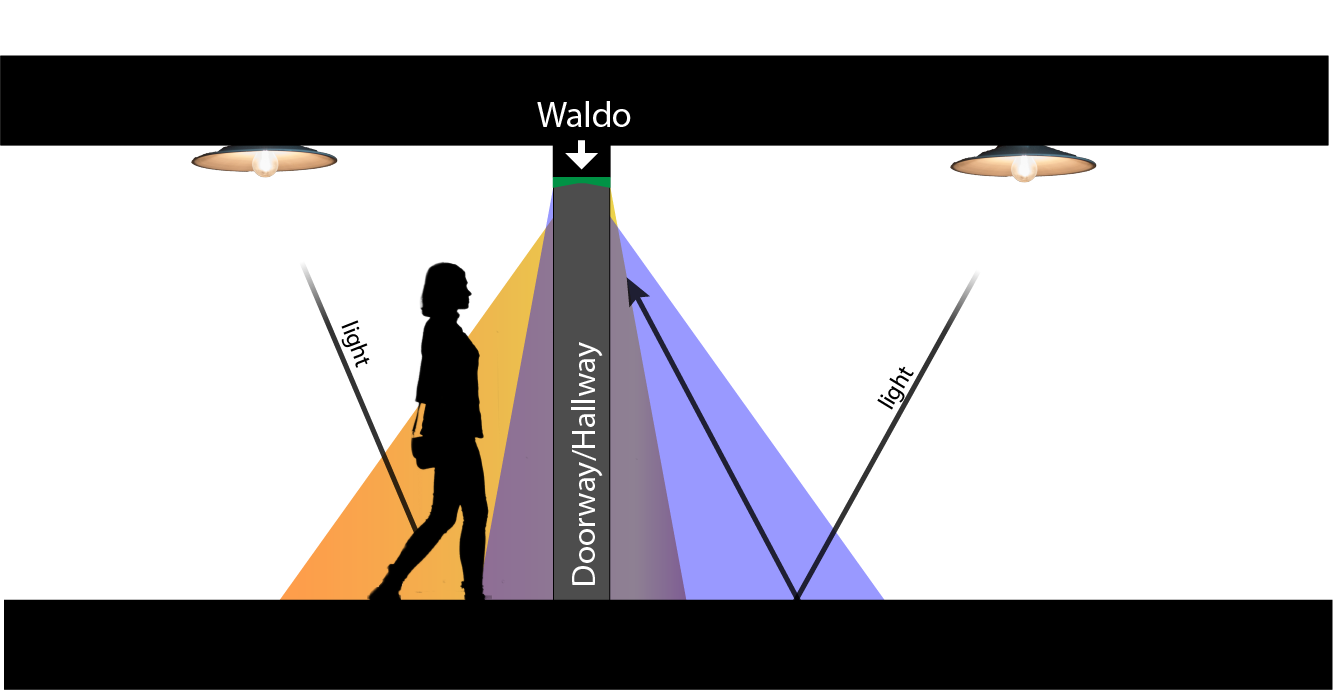
\includegraphics[width=\columnwidth]{figs/scenario2.png}
\caption{ The overall system concept of \sysname, a batteryless, energy-harvesting, doorway mounted occupancy tracking and person detection enabling system.  This system uses reflective indoor lighting to both power the system and detect person entry and exit activity to a room or corridor.\label{fig:syspic}}
\end{figure}
% why batteryless?
%Importantly, \sysname is batteryless to enable the long term deployment at scales required to instrument entire commercial buildings and residential neighborhoods.
%Batteries are expensive, bulky, environmentally unsustainable, and do not have long lifetimes (even rechargeables).
%By leaving the batteries behind, the device power supply becomes intermittent, complicating execution, data collection, energy management, and timekeeping.
%However, the ability for long term deployments at the scales envisioned for the Internet-of-Things provides enough motivation.

Like previous solutions~\cite{hnat2012doorjamb}, \sysname attaches to the top of a door frame and monitors movement in and out of the doorway.
In contrast, however, \sysname does not use active sensors~(like ultrasonic range finders), but instead senses movement using the same ambient light reflections that power the sensor.
\sysname harvests solar energy from indoor lights to power all operations, and uses a combination of hardware and software techniques to detect human movement and direction as solar energy availability changes.
%Besides harvesting solar energy, \sysname processes in hardware and software the signal generated by an array of solar panels to detect when people enter or exit a room.
%When enough energy is available, and a person is walking through the doorway, \sysname uses ultrasonic range finders to measure the height of the person for identification.
\sysname stores this information on device, and opportunistically transmits occupancy information to a basestation using its radio.


%Because of the incredibly tight energy constraints and unpredictable energy-harvesting conditions, \sysname uses approximate computing concepts to provide value to the global system no matter the energy conditions.
%\sysname dynamically adapts its duty cycle, task schedule, and data-transmission granularity, depending on the energy available.
%If relatively high amounts of energy are available in the environment, then \sysname will use the ranging sensor to get heights for each person passing through the doorway, and will send each passing event over the air through BLE to the basestation.
%If relatively low amounts of energy are available in the environment, then \sysname will turn off the range finder, and use only the passive, zero-energy-cost solar panels to detect passing events.
%Instead of transmitting on each passing event in this low energy state, \sysname instead sends global statistics opportunistically, detailing the number of events or people that have passed since the last interaction.


%\subsection*{Contributions}
\noindpar{Contributions:}

%\begin{compactenum}
\begin{enumerate}[label=\arabic*., align=left, leftmargin=*]
	\item We present a novel system design for unobtrusive, long-term, low-cost, zero-maintenance occupancy tracking.
	\item We explore design considerations for batteryless, intermittently-powered sensing systems for detecting ephemeral events that can be broadly applied to other batteryless sensing applications.
	%\item A novel approximate computing method for adapting the duty cycle of batteryless occupancy  sensors depending on energy available, trading off accuracy for energy.
%\fxnote{[We need to reword this - HD]} %  1) record heights, 2) then record each event and report, 3) only report stats of people going in and out
	%\item An investigation of security and privacy considerations stemming from ubiquitous, low cost occupancy sensors.
	\item We provide an implementation, deployment (both controlled and in-the-wild), and evaluation of \sysname that explores the strengths and limitations of our approach. 
%\end{compactenum}
\end{enumerate}

\noind
\sysname is, to our knowledge, the first batteryless occupancy-monitoring solution~\cite{desai2018, sorber_tobias_2022}, and demonstrates the potential and usefulness of long-lived, energy-harvesting, batteryless sensing operation in the built environment. %\fxnote{[I'm waffling between simply saying as we had that we were the first and citing the patent... which is here but also could simply say "the first single sensor batteryless occupancy-monitoring system solution" - could be worded better or maybe I'm just overthinking this.  Let me know what you all think here.  -NT]}
In this paper we present our design, a working prototype, and evaluation results showing the efficacy of the approach.


% These types of condensed table of contents in papers communicate essentially nothing, let's not waste the space - JDH
%\noind
%In the following sections, we give background and related works on occupancy detection and batteryless sensing (\secref{sec:background}), outline the \sysname system design (\secref{sec:system}) and implementation (\secref{sec:implementation}), demonstrate the feasibility and general applicability of \sysname in a variety of situations (\secref{sec:evaluation}), discuss limitations, privacy considerations, and future work (\secref{sec:discussion}), and conclude (\secref{sec:conclusions}).

\section{Batteryless People Sensing}
\label{sec:background}

% Batteryless sensing is needed for large scale because....
Energy-harvesting batteryless sensors are critical to an affordable and sustainable Internet-of-Things~(IoT) and the future of smart buildings.
%
Running wires to power new sensors and other devices is expensive and not always feasible.
On the other hand, batteries are expensive, bulky, and often hazardous.
Even rechargeable batteries wear out after a few years, and replacing trillions of additional batteries every year would be both expensive and irresponsible.
%
In contrast, batteryless sensors powered entirely with harvested energy cost less, weigh less, and can operate for decades with minimal maintenance and environmental impact.

%Long term deployments at scale, like \sysname,
However, batteryless sensing is challenging.
Energy is stored in one or more small, cheap capacitors to improve efficiency and responsiveness~\cite{jhester:ufop:sensys}.
Harvested energy is variable and difficult to predict.
Power failures are common, interrupting computation and data processing, sensing, and communication.
Clocks reset and volatile memory is lost frequently, complicating a developer's ability to build robust and sophisticated applications.

Recent advances in checkpointing~\cite{ransford2011mementos, balsamo2015hibernus}, consistent execution~\cite{colin2016chain, Lucia:2015:Dino}, timekeeping~\cite{hester2016persistent}, energy management~\cite{jhester:ufop:sensys}, testing~\cite{ekho-sensys}, and debugging~\cite{colin_edb} address key challenges and have enabled new and interesting applications. Examples of such applications include  tracking building and appliance energy consumption~\cite{debruin2013monjolo,campbell2014energy} and monitoring greenhouses~\cite{jhester:ufop:sensys}.


In spite of these improvements, current batteryless sensing applications are limited and typically fall into one of two categories: those that depend on an RFID reader and those that opportunistically detect valid, useful data whenever measured.
Power failures and long outages make it difficult or impossible to gather streams of uninterrupted data, inevitably resulting in an inferior quality performance when compared to reliably powered sensors.
This has complicated the design and deployment of such batteryless sensors in many application areas.
%This has led to avoidance of some sensing applications that work best with uninterrupted sensing; such as occupancy monitoring.

Occupancy-monitoring applications try to instrument \fxnote{[Is there a better term besides 'instrument' to use here? -NT]}buildings, people, or other indoor elements to get a better understanding of the number of people in a room.
This information is the baseline data for successful operation of smart building functions such as intelligent temperature and HVAC control, efficiency monitoring, elderly tracking, and other applications.
Existing occupancy-monitoring systems use many sensing techniques and deploy in many different form factors, with doorway-based sensing being one promising method~\cite{hnat2012doorjamb, sonicdoor-buildsys2017}.
In this paper, we implement a doorway-mounted batteryless sensor for occupancy monitoring and investigate the challenges posed by an unreliable power supply to achieving a reasonable quality of sensing.
We recognize three major aspects to implement a successful sensing system with unreliable power:
% What are the challenges for batteryless occupancy sensing beyond the regular challenges?

\noindpar{Intermittence:}
Small energy storage combined with unpredictable energy harvesting means that batteryless devices must be equipped to handle intermittent operation.
Specifically, batteryless occupancy sensing devices must be careful to (1) optimize operation to make best use of available energy, (2) use ultra-low-power techniques and passive methods to perform the actual sensing and support the applications, and (3) be failure resistant, gracefully handling power failures and returning to deterministic states.

\noindpar{Energy harvesters as sensors:}
A sensing system traditionally consists of a dedicated sensor to gather data, along with some form of processing and communication, powered from a reliable energy source.
We propose an alternative to this approach by inferring the signal from variations in the harvested energy, instead of using that energy to power an explicit sensor.  \fxnote{[Maybe breaking up this sentence here as such: "...approach by making use of the collected energy itself as data.  This approach gathers data by inferring... ", just a suggestion to extra enforce the energy as data narrative -NT]}

For example, door-mounted occupancy sensors can harvest energy from indoor and ambient lighting using solar panels pointed towards the floor or other reflective surfaces.
Concurrently, this energy is also a \textit{signal} that can be processed to gain insight into the changing environment of the building, the movement of people and objects, or even the time of day.
We can use this correspondence between energy and data to enable passive sensing and consequently, batteryless occupancy detection.
If a door-mounted entry and exit sensor has solar panels that point down towards the floor, a person walking through the doorway will block some of the light, reducing the energy harvested at that point in time.
This event can be tracked passively, effectively transforming the solar panels into zero-power sensors.
This signal will be affected by the changing power draw of the system (an artifact of the I-V curves of solar panels) and will have a changeable resolution and magnitude depending on the incident light intensity.
These factors make the overall signal noisy; however, careful signal processing in the energy constrained computational environment can provide useful information, freeing up energy that would otherwise have been consumed by an actively-powered sensor (like a PIR sensor or ultrasonic range finder).

\noindpar{Human and building confounds:}
Harvesting both energy and signal from solar panels introduces confounding factors from the variability of lighting in buildings, and the variability of people and their habits.
Many buildings will have some well-lit rooms bordering dim hallways, or vice-versa.
Natural light may be abundant in some rooms, while others have only artificial light.
Also, clothing, hair color, skin color, walking speed, and height will all affect and potentially change the readings on the solar panels.  \fxnote{Maybe include something like...[Humans also have a tendency to complicate data by not strictly walking in and out of a doorway---they like to linger, pass-by, and abruptly change direction, for example.]-NT}
Any system that promises robust occupancy monitoring using energy harvesting must be able to handle these  confounding factors.





% We are not doing any of this now
%\noindpar{Approximate Tasks:} Continuous sensing application require uninterrupted streams of data to ensure no events are missed.
%For occupancy setting, it is observed that it is much better to enable longer streams of uninterrupted sensing at a lower application quality or application accuracy than to gather short, intermittent bursts at a higher quality, requiring more energy, and constraining execution to only a certain level of available energy.
%To support nearly continuous sensing, approximate computing can be leveraged, trading accuracy and quality of services for uninterrupted operation.
%The following are required for this to work: 1)~identifying the levels of service that can be supported by the application, and 2)~knowing when to switch between these levels of service.
%Approximate computing applied to batteryless systems works especially well when sensor data exhibits high temporal locality, meaning that a data point gathered immediately after another may be worthless, as nothing has changed (for example when monitoring an empty doorway).
%Knowing when to reduce the level of service is a key challenge.


% Introduce and bridge to the next section (system design that answers these challenges)
Batteryless occupancy sensing has never been done; but can take advantage of a key observation to provide reliable service---the reality that the applications' harvested energy can also be used a data stream that serves as a sensor.
By taking advantage of the temporal locality of energy harvesting and data in occupancy sensing, we can build a long-lived sensor that detects and identifies the movement of people as they enter and exit rooms.
In the following sections we discuss \sysname, a novel sensing system that demonstrates the feasibility and utility of intermittently powered, energy-harvesting devices, for sensing in the sustainable future Internet-of-Things.

\section{The \sysname Design}
\label{sec:system}
% Basic what it is
\sysname is a slim, batteryless, occupancy-monitoring sensor system mounted to the top of a doorframe.
It is powered by energy harvested from two arrays of indoor solar panels pointed at the floor.
The panels serve two roles: 1)~energy harvester and 2)~sensor.
These panels gather \textbf{energy} for computation, sensing, and signaling while also providing the \textbf{signal} that \sysname uses to detect when a person walks through the doorway in the form of variations in the harvested energy.
\sysname records the direction---entry or exit---of each doorway event and stores this information in non-volatile memory for later transmission.


\noindpar{Design Goals:} Unpredictable power supplies and human behaviors make designing an intermittently-powered occupancy sensor challenging.
We designed \sysname to meet the following design goals. 

%uncomment to save a few lines.
%\begin{enumerate}[wide, labelwidth=!, labelindent=0pt]
\begin{enumerate}
	\item \textbf{Availability:} Doorway events can occur at any time.
	While many intermittent sensors gather data opportunistically as energy is available, \sysname is designed to conserve its harvested energy so that it is available to detect ephemeral doorway events, whenever they occur.
	\item \textbf{Accurate direction:} In addition to detecting someone passing through the doorway, \sysname uses angled solar panels to accurately determine their direction.
	This plays a crucial role in inferring the occupancy of rooms and buildings.
	\item \textbf{Variable lighting conditions:} Indoor lighting conditions can change over time, due to human behavior and the relative movement of the sun.
	We have designed \sysname to work in a range of different lighting conditions by using detection circuits that respond to changes in light level, independent of the absolute amount of light, as well as tuning mechanisms built into the prototype.
	\item \textbf{Variable human characteristics:} An effective occupancy sensor should work well in spite of variations in clothing, hair, height, walking speed, and skin color. By focusing on changes in total reflected light, \sysname is robust to these human variations.
	\item \textbf{Form factor:} We want \sysname to be easy to deploy, to fit unobtrusively inside a door frame, and avoid contact with doors (on frames with doors).
	We could harvest more energy by wrapping \sysname around the doorframe, but the system would be more expensive, harder to deploy, and more likely to interfere with doors, while also changing the aesthetics of the doorway.
\end{enumerate}

\noindpar{What \sysname is not.}
We also want to be clear about what \sysname is \emph{not}.
\sysname is \emph{not} a security device.
\sysname helps building owners and managers understand how people move through buildings, but it is \emph{not} designed to thwart malicious behavior.
We can easily trick \sysname with a flashlight or reflective materials, and we can disable it completely by covering its solar panels or turning off the lights.
Users looking to prevent shenanigans or tomfoolery should use a different device.
Users looking for a long-lived, low-maintenance, best-effort batteryless occupancy sensor for monitoring normal behaviors should read on.

% fig refs
\noindpar{}
The \sysname hardware architecture, shown in \figref{fig:overview}, includes support for energy harvesting, event detection, computation, and communication.
% Intro the rest of the section
In this section, we describe these components and how they work together to meet \sysname's design goals.


\begin{figure}[t]
\centering
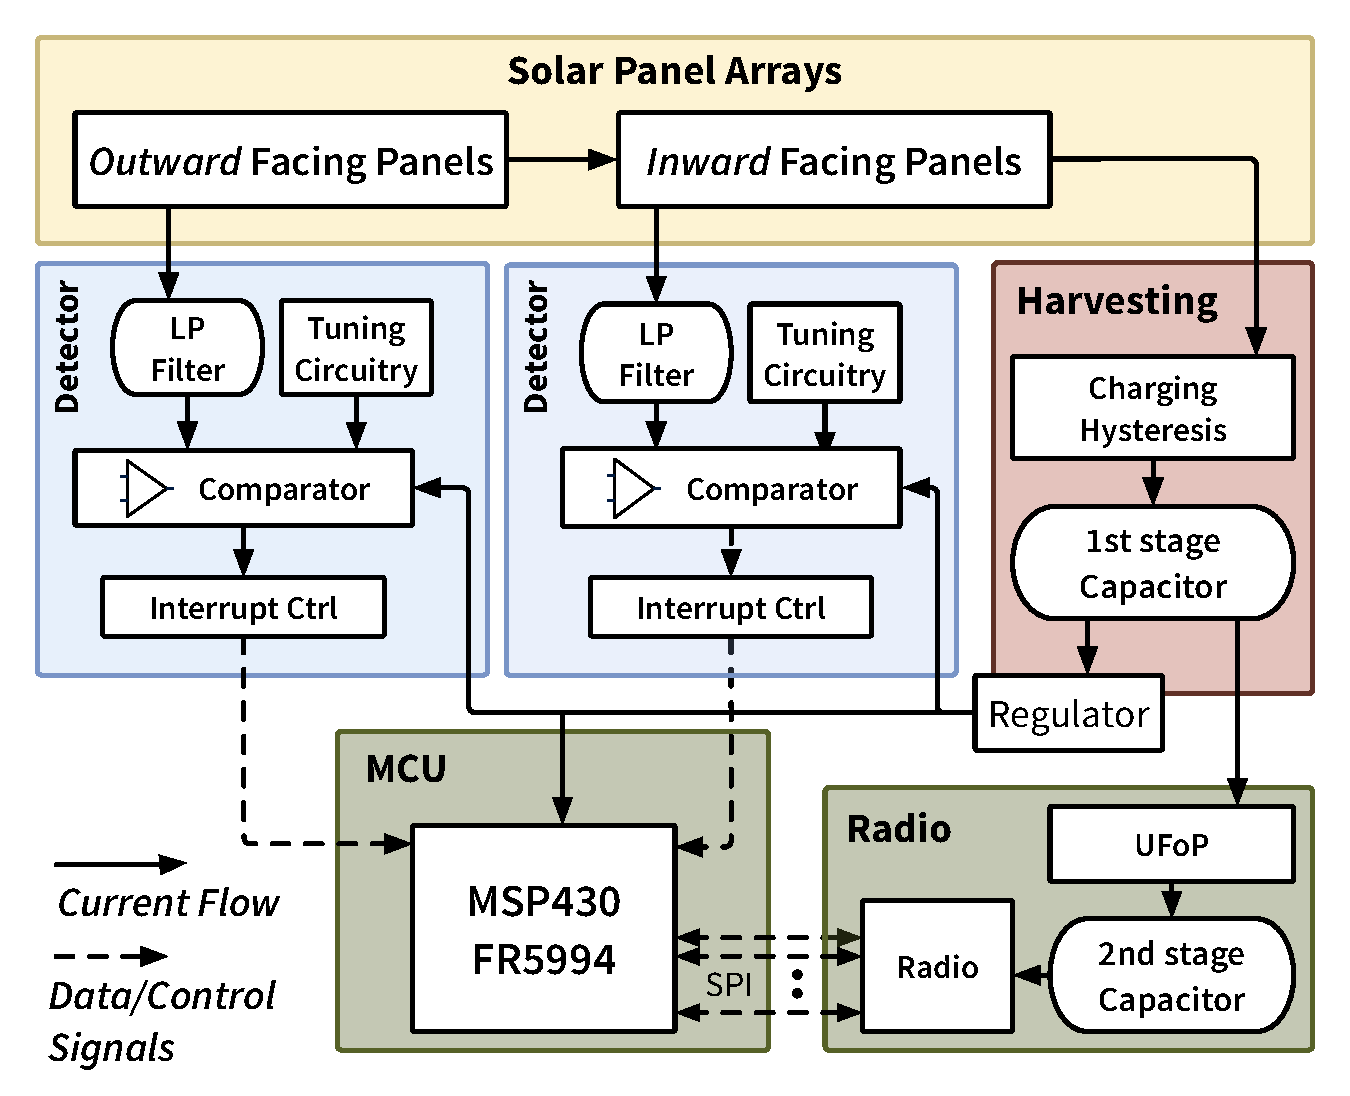
\includegraphics[width=\columnwidth]{figs/overview.pdf}
\caption{The \sysname architecture overview. \sysname uses the energy and signals from two sets of solar panels to both power the sensor and detect people passing into and out of a doorway. Two detector circuits each monitor the solar panels sets mounted in series in the doorway. One detector monitors a set of similarly facing panels, while the other observes the combined signal from all of the panels. On detection, the detectors wake up the MCU to process, log, or communicate occupancy information.  \label{fig:overview}}
\end{figure}


\subsection{Energy Harvesting and Management}
\sysname takes advantage of the ubiquity of indoor light in homes and offices.
Solar panels are mounted to the top of the door frame, pointing down toward the floor---half tilted \ang{20} inward and half tilted \ang{20} outward.
Pointing the panels downward is not ideal for energy harvesting but effective for detecting doorway events and provides a slim, easy-to-deploy unobtrusive form factor.
Tilted panels help \sysname determine walking direction, since a person will affect one half of the panels before the other. 
%\fxnote{[Not sure if this needs to be reworded since half of the panels might not accurately represent what is going on here.  Maybe instead -- will trigger one of the detectors at varying times, or something like this.-NT  The statement is true, and clarified in the next paragraph. This is fine. -JMS]}

To maximize energy harvesting, we connect the two sets of solar panels---the inward-facing set and the outward-facing set---in series.  
A series configuration conveniently combines the two panel sets into a single power source that can be used without adding boost regulators or other power conditioning circuitry.
This configuration makes it more difficult to analyze the two signals independently since they lack a common ground\footnote{For a series connection, we connect the positive terminal of the first panel set to the negative terminal of the second.}.
Instead, we measure the voltage of the outward-facing set alone, and the combination of the two sets.
We could compute the inward panels' voltage by subtracting the two; however, we have found that we can skip this step and just compare the two measurements directly, as shown in \figref{fig:traces}, to determine walking direction.


\sysname uses federated energy storage~\cite{jhester:ufop:sensys} to power its microcontroller and peripherals.
Harvested solar energy is fed into a common first-stage storage capacitor and then automatically federated to its one peripheral---a Texas Instruments CC1101 radio.
Federating energy allows us to start detecting and processing events while saving up energy for more energy-expensive radio transmissions.
It also improves harvesting efficiency and reduces the risk that the microcontroller will lose power due to a radio transmission.

\begin{figure*}[t]
	\centering
	\begin{subfigure}[b]{0.45\textwidth}
		\centering
		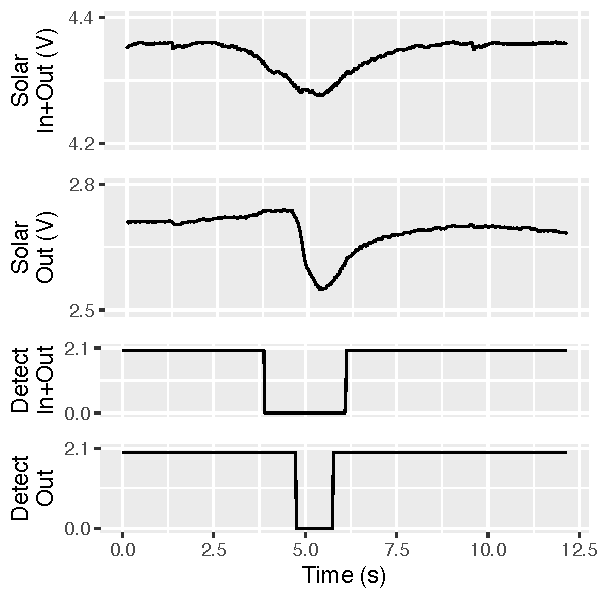
\includegraphics[width=0.8\columnwidth]{figs/tracesin.pdf}
		\caption{Walking in.}
		\label{fig:tracesin}
	\end{subfigure}%
	%
	\begin{subfigure}[b]{0.45\textwidth}
		\centering
		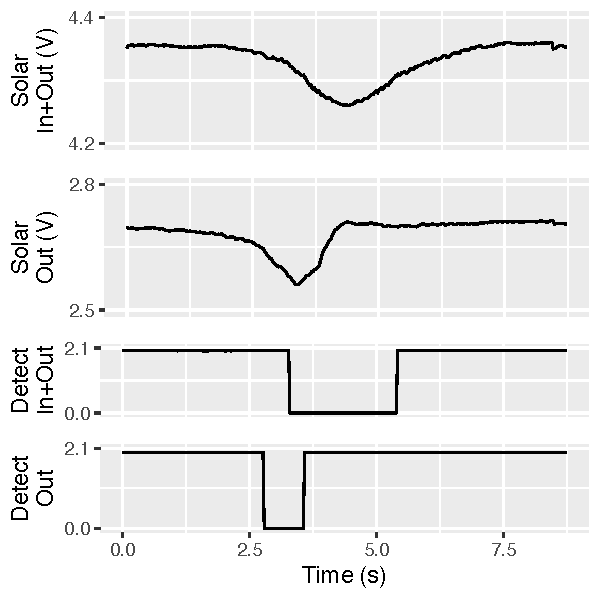
\includegraphics[width=0.8\columnwidth]{figs/tracesout.pdf}
		\caption{Walking out.}
		\label{fig:tracesout}
	\end{subfigure}
	\caption{These traces show example solar panel voltages and detector outputs over time when a person walks through a \sysname-enabled doorway. The top traces show how the solar panel's voltages are deformed during the doorway event. The detector triggers are used to wake up the microcontroller and detect events and their direction. The angling of the panels cause the inward facing and outward facing detectors to trigger at different times depending on the direction the person is walking.\label{fig:traces}}
\end{figure*}

\subsection{Detection}
\label{sec:detection}



%\fxnote{[It would be nice to do this data driven off some traces gathered. Simulate, essentially, just by doing some light math. So how do we capture the waveforms when we trigger the wakeup? - JDH]}

%what happens when a person walks through.
When someone walks under \sysname, they block some of the reflected light hitting the solar panels.
In \figref{fig:traces}, the solar traces on top show how solar panel voltage changes during a doorway event.

In order to detect a doorway event, we could use an ADC to continuously measure the solar panel voltage over time and analyze those readings to detect the presence and, more importantly, direction of motion.
Voltage levels and waveform shapes vary with lighting conditions, especially when one side of the doorway has more natural light.
This approach would mean more complicated signal analysis and much higher energy consumption.
Instead, \sysname uses a \textbf{detection circuit} that wakes up the microcontroller when it detects a significant change in the solar panel voltage over a short period of time.
This circuit consists of a passive first-order capacitive filter connected to a nano-power comparator---producing a square wave that transitions when the voltage increases or decreases faster than a set rate.
These transitions trigger interrupts that help \sysname detect when someone is passing through the doorway.

In order to determine movement direction, we use two detector circuits: one that detects change on the outward-facing panels and another that detects change on the combined inward- and outward-facing panels.
When someone walks through the doorway, the detectors trigger at different times, depending on the walking direction, as shown in \figref{fig:traces}.
\sysname compares the timing of these detector interrupts to distinguish incoming and outgoing events.


\noindpar{Removing light flicker.}
Many fluorescent indoor lights flicker at \SI{60}{\hertz} or higher---a much higher frequency than the events \sysname detects.
If not filtered out, fluctuations can confuse the detection circuit and produce false positive results.
We add a low-pass filter to remove noise above \SI{10}{\hertz} from the solar panel signal.

\noindpar{Isolating harvesting from sensing.}
If connected directly, \sysname's harvesting and event detection circuits can potentially conflict in two important ways.
First, the harvesting circuit stores harvested energy in a \SI{100}{\micro\farad} capacitor---a size that ensures that \sysname can store enough energy for short-term tasks and dampens the low-frequency voltage fluctuations that we need in order to detect doorway events.
Second, short-term power spikes from interrupt service routines and other computation cause high-frequency dips in the solar voltage, which can confuse the detection circuits.
We address both of these challenges by adding an additional low-pass filter between the detection and harvesting circuits. This isolates the solar panel from the load, and allows the solar panel voltage (after the initial flicker filter) to fluctuate over a wider range in response to doorway events with less interference from the storage capacitor, the microcontroller power draw, and the detector circuit power draw. 

\noindpar{Detection algorithm:}
\sysname's software works as shown in \figref{fig:software}. 
During normal operation, when no doorway events are detected, \sysname's MCU remains in a sleep mode, only waking up to report heartbeats after two minutes of inactivity.
While in sleep mode, the MCU only wakes up in two cases: 1)~when its inter-event timer fires (this timer measures the time that has passed since the last reported event) and 2)~when activity near the sensor triggers the detector circuits.
A detector transition from a high state to a low state---due to a drop in harvested solar energy caused by a person walking through the doorway---will wake up the system to process an event.
This initial wake-up marks the start of an event.
The MCU records when the interrupt occurred, starts an event timer~(6 seconds), and goes back into sleep mode.
During the \SI{6}{\second} event, the MCU will wake up each time the detectors transition (from HIGH to LOW and vice versa) to record the length of time between each transition.
A person may block light in many ways, and so multiple interrupts may fire during a single doorway event.
When the event timer fires (after \SI{6}{\second}), the event is considered finished and event classification and recording begins.

\begin{figure}[t]
\centering
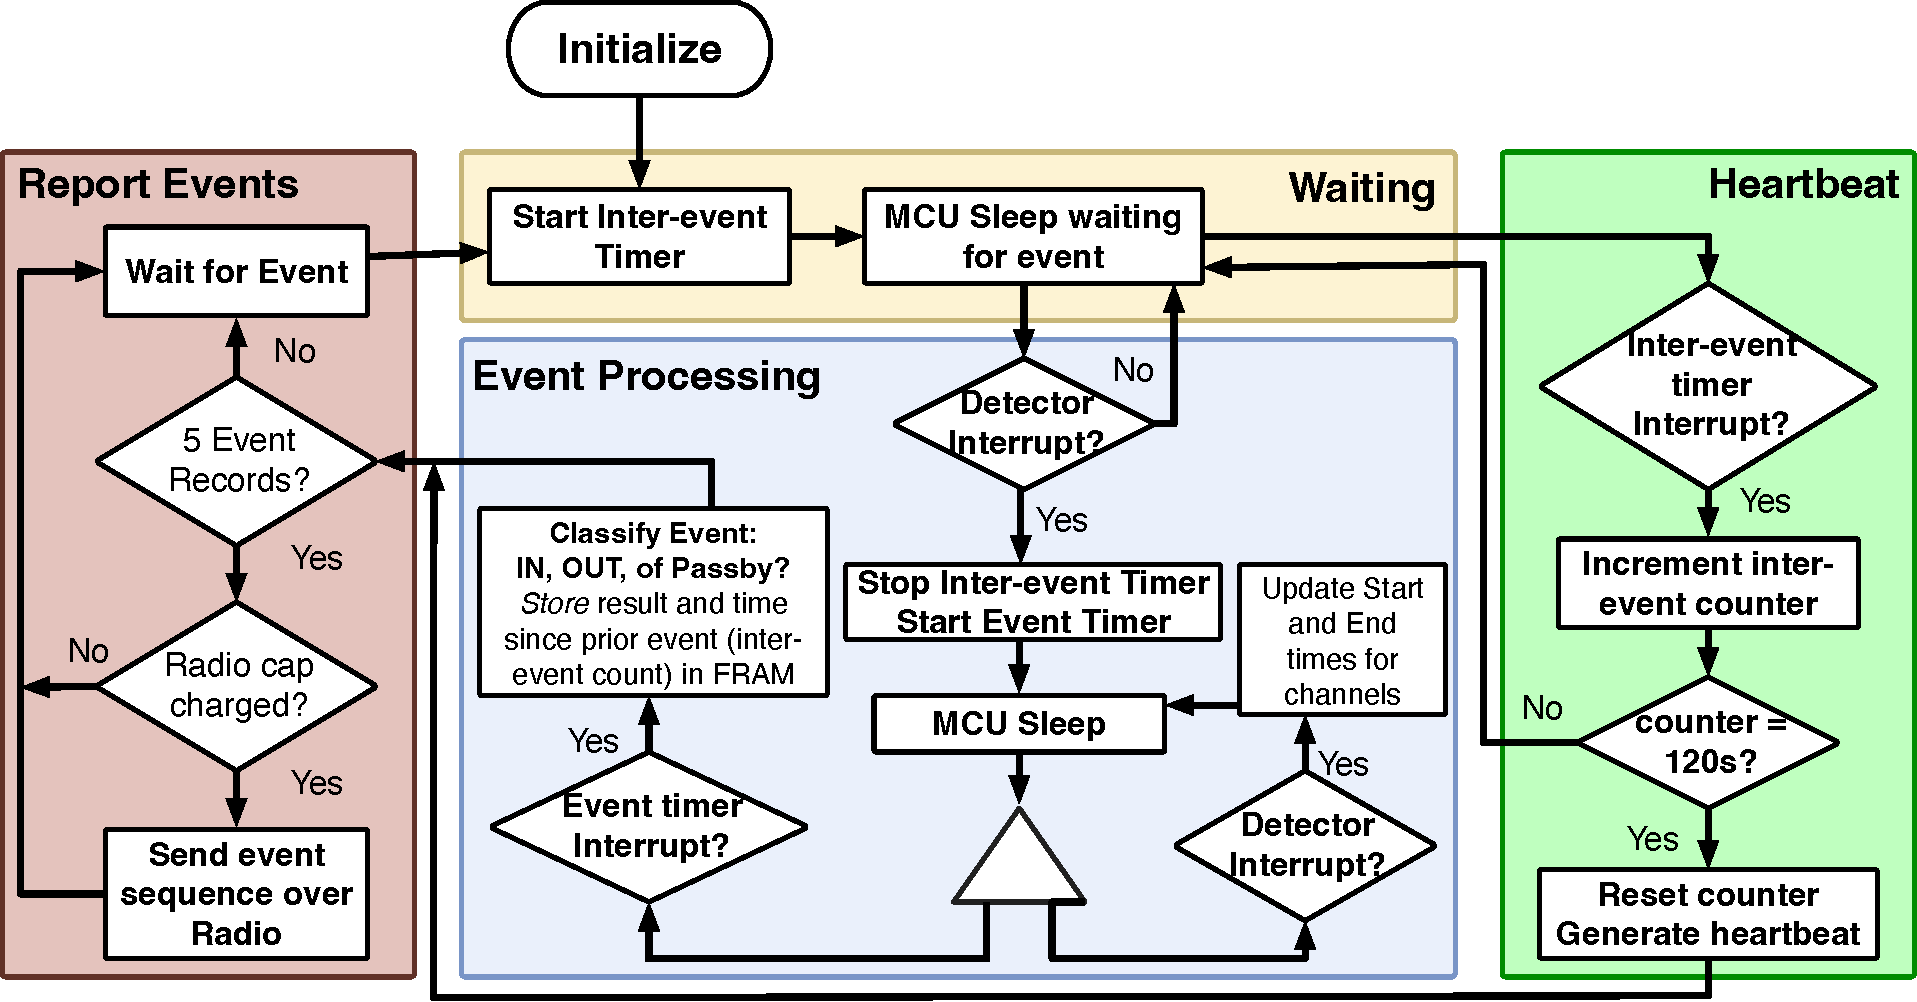
\includegraphics[width=\columnwidth]{figs/software_update.pdf}
\caption{The \sysname detection algorithm and system decision flowchart. The algorithm is composed of four parts that handle reporting doorway events, processing detected events, processing time between events and heartbeats, and idle waiting. \label{fig:software}}
\end{figure}


Times are recorded for the first falling edge interrupt (start time) and the last recorded rising edge (end time) for both solar panel sets of inward and outward facing panels.
When the event timer fires, the system has recorded both solar panel sets' start and end times, which are the features used to classify the event.
%For initial testing, we simply compare these times to determine the direction of the event (entry or exit), and the \sysname stores the detected event in non-volatile memory.
For training, we collected features from 332 controlled events from two different people at three different locations, a lab, an office, and a hallway.
Using this data, we trained a 4-layer decision tree that classifies events as INs, OUTs, and PASS-BYs (when a person passes within a few feet of the sensor, but not under it.)
When locations had a door, the door remained open for the collection.  %
% These events allowed us to not only train the system on standard ins and outs, but also on variations of passing by a doorway (a foot away to a couple of feet away on both sides of the system) which could trigger false ins and outs in the system.  A 4-layer decision tree was trained on 70\% of the events and tested on the remaining ones - achieving a 93.25\%-94.38\% accuracy.  
The trained decision tree is then used on \sysname to classify observed events during deployments.  


Between events, \sysname uses an inter-event timer to estimate time between events.  
When the next event is detected, the inter-event timer is stopped and then the event timer is started for processing the event interrupts during the event window.
A heartbeat record is generated when the time since the last event passes 120 seconds and is added to packet information to be sent with other records to the basestation. 
Once the event is processed and classified or heartbeat is generated, it is recorded in non-volatile memory along with the estimated time that has past since the last event or heartbeat record.  
The inter-event timer is then reset and the cycle continues.


\subsection{Communication and Infrastructure}
\sysname's collected data are stored in non-volatile memory until the system has saved up enough energy to transmit.
To reduce transmission cost, we summarize the last~5 recently-detected event records, sending the sequence of events in order of when they were recorded with the estimated time since the last event that was seen and the classification of that event as an in, out, passby, or heartbeat when 2 minutes of inactivity is recorded.
We compute a CRC over each sequence summary and send the prior two sequence summaries in each packet to reduce the risk of losing information due to corrupted or missing packets and increase the likelihood that a basestation will receive the data. 
If the radio's capacitor isn't sufficiently charged, \sysname will sleep and try again when the next event occurs.
This pattern continues throughout the system's operational lifetime.

%\subsection{Adaptation}
%\fxnote{[Remove this - JDH]}

%\sysname dynamically changes task sets depending on energy availability - attempting to assign higher energy tasks when energy is more available in the environment and assigning lower energy tasks assigned when energy is scarce in the environment. \fxnote{[Does not do this, need to remove - JDH]}
%These tasks correspond to different tiers of quality of service (QoS) of the application, with the highest level providing real time event marking on door traffic coupled with person identification using heights, hair color, and wardrobe. \fxnote{[Does not do this either, need to remove - JDH]}
%The lowest QoS tier corresponds to only logging entry and exit, and sending a summary of the data opportunistically over the radio. \fxnote{[Does not do this either! Put in future work- JDH]}

\section{Implementation}
\label{sec:implementation}

\begin{figure}[t]
    \centering
    \includegraphics[width=\columnwidth]{figs/full_waldo_open_cropped.png}
    \caption{3D printed solar panel and PCB housing enclosure with angled slots for solar energy harvesters and the \sysname prototype PCB.}
    \label{fig:mounting}
\end{figure}    

%\begin{figure*}[t]
%    \centering
%    \begin{subfigure}[b]{0.5\textwidth}
%        \centering
%        \includegraphics[width=\columnwidth]{figs/full_waldo_open_cropped.png}
%        \caption{3D printed solar panel enclosure with angled slots for solar energy harvesters.}
%        \label{fig:mounting}
%    \end{subfigure}%
    %
%    \begin{subfigure}[b]{0.5\textwidth}
%        \centering
%        \includegraphics[width=0.75\columnwidth]{figs/waldoguts-anon-white.png}
%        \caption{ \sysname prototype PCB.}
%        \label{fig:pcb}
%    \end{subfigure}
%    \caption{\sysname implementation \label{fig:prototype}}
%\end{figure*}

In order to evaluate our approach, we implemented a prototype \sysname sensor that includes custom hardware (shown in \figref{fig:mounting}), firmware for detecting and reporting doorway events, and a custom 3D~printed doorway mounting system that holds the assembled PCB and solar panels in a slim profile~(\figref{fig:mounting}).

\noindpar{Hardware:} Our prototype hardware integrates four~(4)~RL-55x70 solar panels~(70.00mm x 55.00mm) and custom printed circuit boards~(PCB) housed in a 3D-printed plastic enclosure.
The prototype uses an MSP430FR5994 microcontroller from Texas Instrument's~(TI) FRAM line of ultra-low-power processors.
The newest FRAM-based MSP430s have several advantages over previous models: lower sleep-mode currents, shorter wake-up latencies, and faster non-volatile FRAM.
Entirely interrupt-driven and remaining asleep most of the time to conserve energy, \sysname benefits from these improvements.
The solar panels are connected in two angled series-connected banks, each consisting of two series-connected panels.
We connect the panels in series to increase voltage to allow \sysname to work in a wider range of lighting conditions and make doorway events easier to detect.
Our panels---chosen to provide flexibility during prototyping---provide enough current to power the circuit with sufficient voltage levels for detection under a wide range of lighting conditions.
Future designs will focus on miniaturization.
The detector circuitry is made using nano-power comparators (TI~TLV3691) and a passive RC filter network. In order to give us flexibility, the RC filter network is tunable using trim potentiometers pre-installation or digital potentiometers in deployment.  
The \sysname PCB also has a TI~CC1101 radio for communication.
The hardware used in the \sysname prototype, shown in \figref{fig:mounting}, is not prohibitively expensive or obtrusive.

\begin{table}[t]
\footnotesize
\begin{tabular}{@{}p{2.4in}rp{0.1in}r@{}}
\toprule
\textbf{Components}          & \textbf{Cost per unit} & & \textbf{Unit Cost for 1000} \\ \midrule
\textit{Solar Panels}       	& \$ 1.95	& &  \$ 1.76	 \\
\textit{Microcontroller (MSP430FR5994)} & \$ 8.04 & & \$ 5.09	\\
\textit{CC1101 Wireless RF Transceiver} & \$ 9.40	& & \$ 9.40	\\
\textit{Components} & \$ 17.02	& & \$ 6.63     \\ 
\textit{PCBs*} & \$ 2.94	& & \$ 0.30     \\ \midrule
\textit{Entire \sysname Prototype} & \$ 39.35 &	& \$ 23.18    \\ \midrule
\end{tabular}
\caption{Breakdown of the \sysname prototype costs at time of purchase for development.}
\label{tab:costbreakdown}
\end{table}

The total cost of the current prototype at the time of purchase, including all PCBs, component parts, Radio modules, and solar panels is \$23.18 per unit if ordered in quantities of 1000\footnote{PCBs priced by \url{seeedstudio.com}.}.
The distribution of the prototype costs are showed in Table~\ref{tab:costbreakdown}.
The current prototype has several components that are meant to enable experimentation and testing (modular board design, jumpers, headers, test points, etc)---a commercial version of \sysname will be dramatically cheaper and smaller.



\noindpar{Firmware:} %This is now up2date -NT 4/1
The \sysname firmware implements the detection algorithm with a trained decision tree for event classification discussed in \secref{sec:system}.
Monitoring the interrupts from the detectors and deducing the direction of motion upon triggering are the main tasks of the system.
The firmware is designed to be ultra-low power, even in active mode, and has low computational complexity, offloading the bulk of the detection to the hardware circuits.
The \sysname firmware is composed of 691~lines of commented C code, compiling to a 4459~byte image. This code size comprises only 1.7\% of the available code space on the MSP430FR5994~(256KB), leaving ample room for implementing custom tasks, recognizers, or multiprogramming operating systems.

\noindpar{Mechanical Design:} %Dimensions are current-NT 4/1
The 3D printed mounting system (shown in \figref{fig:mounting}) is made of PLA plastic and contains the PCB, solar cells, and necessary wiring connecting them.
\sysname's 3D printed enclosure measures \SI{56.0}{\milli\meter} by \SI{395.9}{\milli\meter} by \SI{22.8}{\milli\meter} at its thickest point. The enclosure provides a nesting place for the solar cells, pointing downward. 
A simple slide-mounted cap was also designed to cover the PCB housing to help minimize distractions when deployed.  The sensor could be minimized further by selecting smaller solar panels and by placing the PCB behind the panels rather than to the side of the panels.
The angle of the solar cell slots is set such that half of the solar cells tend toward the entry, while the rest face toward the exit.

All software, firmware, hardware schematics and layouts, and 3D printed mounting system will be made freely available at publication time.

\section{Evaluation}
\label{sec:evaluation}
In order to evaluate the efficacy of our approach, we evaluated \sysname in both controlled and in-the-wild deployments.  

\subsection{Controlled Experiments} 
We evaluated \sysname's performance under controlled conditions in three phases to test different variables the system might encounter:

In \textbf{phase one} we tested \sysname on multiple doorways, with different characteristics---light levels, flooring, doorway heights and doorway widths.
For each test, we primarily evaluated \sysname's ability to detect someone passing through and determine the person's direction of movement.
We also tested the system's robustness to human variation, like height, clothing, and hair color by including a diverse group of subjects.
We tested on \numDoors different doorways with \numPeople people for a total of \numExp different doorway events (each person walked through multiple times per doorway).\footnote{This study was approved by our Institutional Review Board.}

In \textbf{phase two} we test the limits of the device, examining the factors that affect its accuracy, performance, and availability---including lighting conditions, walking speed, and short delays between doorway events.
We also tested a variety of events that may be falsely detected as doorway events.

In \textbf{phase three} we explore the energy harvesting ability and gather microbenchmarks of the energy consumption of the parts of the \sysname system.

\begin{table*}[t]
\footnotesize
	\begin{tabular}{@{}p{0.6in}p{0.5in}p{0.5in}p{0.45in}p{0.6in}p{0.3in}p{0.7in}p{0.7in}p{0.5in}@{}}
	\toprule
	\multirow{2}{*}{\textbf{Doorway \#}}	&	\multicolumn{2}{c}{\textbf{Light Intensity (lux)}} & \multicolumn{2}{c}{\textbf{Flooring}} & \multicolumn{1}{c}{\textbf{Enough}} & \multicolumn{1}{c}{\textbf{Total}} & \multicolumn{1}{c}{\textbf{Detection}} & \multicolumn{1}{c}{\textbf{Direction}} 		\\
	& Inside & Outside & Inside & Outside & \multicolumn{1}{c}{\textbf{Light?}} & \multicolumn{1}{c}{\textbf{Events \#}} & \multicolumn{1}{c}{\textbf{Accuracy(\%)}} & \multicolumn{1}{c}{\textbf{Accuracy(\%)}}\\\midrule
	1 & 86 & 96\textsuperscript{*} & Tile & Tile & Yes & 162 & 93.82 & 98.02 \\ %Lab Door
	2 & 86\textsuperscript{*} & 64 & Carpet & Tile & Yes & 63 & 90.48 & 78.94 \\ %224
	3 & 71 & 55 & Carpet & Tile & Yes & 106 & 100 & 98.11 \\	%Jacob's office
	4 & 96 & 111\textsuperscript{*} & Tile & Tile & Yes & 106 & 100 & 98.11 \\ %232
	5 & 55 & 55 & Tile & Tile & Yes & 112 & 99.1 & 94.59 \\ %hallway1
	6 & 55 & 71 & Tile & Tile & Yes & 102 & 100 & 96.08 \\\midrule %hallway2
	7 & 40 & 71 & Carpet & Tile & No & - & - & - \\ %226-1
	8 & 24 & 72 & Carpet & Tile & No & - & - & - \\ %226-2
	9 & 24 & 55 & Tile & Tile & No & - & - & - \\ %hallway-119
	\bottomrule
	\end{tabular}
	\caption{Evaluation results with 12 test subjects having variable heights, hair color, and clothing as described in \secref{sec:normal_operation}. We tested 9 different doorways, from which 6 had enough light to power \sysname. We ran multiple people through each of these 6 doorways, noting the detection accuracy and how many of the detected events had correct direction. These results show that an adequately-lit \sysname occupancy monitor can accurately detect doorway events and their directions.
	\vspace{1mm}
	\\\textsuperscript{*}Mixed Lighting --- Combined natural and artificial light
	\label{tab:detection}}

\end{table*}



\subsubsection{Methodology and Claims}
The following experiments address the goals defined in \secref{sec:system}.
We address system availability~(Goal~1) by demonstrating the low power draw of the system itself and the number of times it caught doorway events (and the number of doorway events missed) for each doorway test.
% the minimum light intensity at which \sysname can sustain operation and detect doorway events.
Further, we evaluated the accuracy in determining the direction~(Goal~2) by observing how often \sysname correctly determined walking direction.
We explored variable lighting conditions~(Goal~3) by testing the device under \numDoors different doorways with diverse lighting conditions, both typical and adverse.
We address human variation~(Goal~4) by evaluating different walking speeds and the effect of clothing and hair color/hair covering on detection patterns.
We claim that~(Goal~5), concerning form factor, is addressed by our prototype and slim mechanical design, described in \secref{sec:implementation}.

We also tested the limits of the device, by varying different factors to see when the device stops working and generating conditions that can confound the sensor.
These tests cannot hope to cover all possible deployment conditions, but they do give a broad sense of the capabilities and limitations of \sysname.

We gathered all electrical signal measurements, except where specified otherwise, using the Saleae Logic~16 logic analyzer\footnote{https://www.saleae.com} at a sampling rate of 5KS/s.
The analyzer's high impedance ADCs allow for unobtrusive signal monitoring.
This sampling rate is sufficient to detect the types of slow-varying doorway events that human activities produce.
We manually recorded the direction of each doorway event as ground truth to verify the accuracy of \sysname in event detection, then compared the ground truth results with the results measured by the logic analyzer.
We measured light intensity levels using a TSL2561 Light-to-digital converter,\footnote{https://cdn-shop.adafruit.com/datasheets/TSL2561.pdf}
aligned to the same angle as the solar panels in both directions to get accurate light intensities falling on the panels.

Finally, we note that it is difficult to fairly compare the performance of different occupancy-monitoring systems except in their accuracy. For example, CeilingSee~\cite{yang2017ceilingsee} uses 16 devices to instrument a room, while \sysname and SonicDoor~\cite{sonicdoor-buildsys2017} place one device in the doorway, and AURES~\cite{shih2016aures} places a single device in the middle of a room. 
For this reason, we investigate the accuracy of \sysname against our manually gathered ground truth (visually verifying a person entering or exiting the room) instead of comparing to another occupancy-detection system.

%%only if time allows:
%%%passing vs. normal entering and exiting of the room
%%%what multiple people entering in close succession looks like to the system and can the system tell the difference between the systems.

%Notes on current testing plan environment:
%tile floor, semi reflective
%door open
%lights on on both sides of the door
%16 solar panels that are alternatively tilted by 10 degrees in either direction (8 panels on each side)
%walking at normal speed through the center of the doorway

%In order to test how well \sysname fares in terms of the availability goal, we tried turning down the light levels till \sysname stopped sustaining operation. Our aim in performing this experiment is to find a threshold above which \sysname sustains operation and is available for detecting ephemeral doorway events as they occur.
%We found that \sysname stops sustaining operation below XXYYZZ lux. This is an acceptable threshold as the average light levels in office environments will be greater than or equal to \SI{70}{\lux}. Even when the light levels fall significantly lower till \SI{40}{\lux}, we are able to detect events but it does affect our direction detection, as outlined in the next section.


\subsubsection{Normal Operation}
\label{sec:normal_operation}

In order to evaluate how well our approach detects doorway events, we tested \sysname across multiple different doorways with a diverse group of subjects.
In these tests, we focused on detecting doorway events caused by a person walking \textit{under} the doorway and accurately determining the direction of the person's movement.

\noindpar{Experiment Overview:}
We tested twelve~(12) different participants, with different physical characteristics---heights ranging from 5'4'' to 6'4'' and hair color ranging from blond to brown and black.
Our test group included a wide range of clothing colors (light and dark) and a variety of head coverings.


For this experiment, we affixed the \sysname prototype to the top of \numDoors different doorways.
\tabref{tab:detection} describes the doorways, including details like light intensity levels and flooring type.
For each doorway, we maintained test subject diversity, in order to characterize \sysname's performance, independent of the characteristics of individual subjects.
For doorways with doors, the door remained open throughout the experiments.
%This was done since
Each participant walked in and out of the room five times in each direction.

\noindpar{Results:}
The results of this experiment, including 651 individual doorway events, are shown in \tabref{tab:detection}.
Each \textit{event} consists of one person walking through one doorway one time.
\sysname successfully detected doorway events and the direction people were traveling through the doorway, detecting a total of \numDet events out of \numExp, giving an overall detection accuracy of \SysAccuracy.
Furthermore, it determined the walking direction correctly for a total of \numDir events, which is \dirAccuracy of the total events detected.
\sysname's performance was consistent across all test subjects, independent of human variations like height, hair color, and clothing.



\subsubsection{Factors affecting \sysname's operation}
\label{sec:confounding}

%\noindpar{Experiment Goals:}
In addition to testing ``normal'' walk through conditions, in this section we examine factors that affect \sysname's performance as an occupancy-monitoring sensor.
It would be impossible to exhaustively study all possible variations, but we are able to explore how \sysname reacts to a variety of conditions and behaviors that it will encounter in actual deployments.
Specifically, we explored the following factors:


\paragraph{Light intensity:}
We tested \sysname on a variety of doorways with varying lighting conditions, with results listed in \tabref{tab:detection}. 
Since \sysname's solar panels are sensitive to visible light and the IR spectrum, we used a TSL2561 sensor to measure both mixed signal (visible and IR) data along with purely IR data, and outputs the combined illumination value in lux.
As shown in \tabref{tab:detection}, our current prototype is fully functional on doorways with light levels above at least 55~lux on both sides.
An average room/hallway in an office-style setting has light levels around 70~lux, which is sufficient to power the \sysname sensor.
It is worth noting that we can customize \sysname for exceptionally dark doorways either by increasing the number of solar panels without changing the working of the system itself, or by employing input booster circuits like the ones used in CleanCut~\cite{colin2018cleancut}.

\paragraph{Walking Speed:}
\sysname detects people walking under doorways based on the changes they induce in the system's harvested energy supply.
This means that if a person walks slowly enough, their movement should become imperceptible to the system.
In order to evaluate this limit, we asked test subjects to walk under the sensor at different speeds.
We used a metronome to which the subjects could match their steps in order to achieve a consistent even speed.
With extremely slow walking (slower than 1~ft/s), we did observe decreased accuracies.
\sysname occasionally detected a slow-moving doorway event as two events.
No test subjects have yet been able to walk slowly enough to avoid detection entirely.
We don't consider this to be a problem for \sysname, since in practice, people don't often move at such slow speeds.

\paragraph{Door Width and Height:}
All doors except door \#4 (in \tabref{tab:detection}) were 80 inches tall, door \#4 was 87 inches tall. 
All doors except door \#6 were 34.5 inches wide, while \#6 was 58.5 inches wide.
A typical interior doorway is 32 inches by 80 inches.
In our experiments, the door width and height had no significant effect on the accuracy, however, we only tested when a single person went through a wide door, and we did not control for participants walking through the middle or side of the door (they were asked to walk naturally).


\begin{figure*}[t]
    \centering
    \begin{subfigure}[t]{0.38\textwidth}
        \centering
        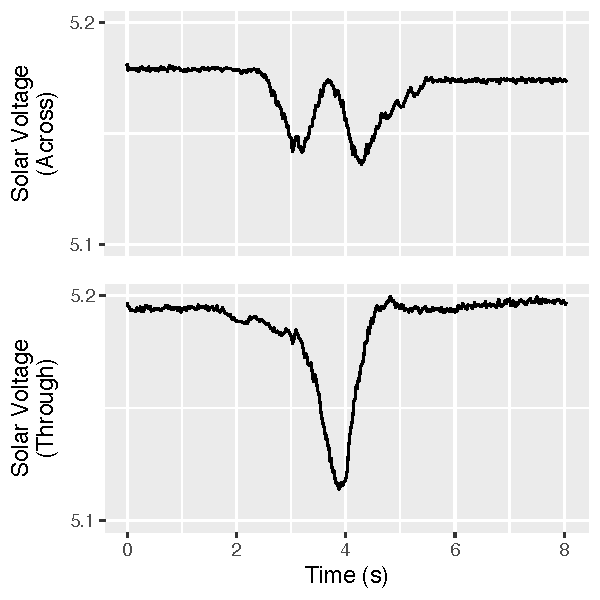
\includegraphics[width=\columnwidth]{figs/spotlight.pdf}
        \caption{These traces show the solar panel output in the presence of the ``Spotlight'' effect. The top figure shows the response when someone walks \textit{across} the ``Spotlight'', while the bottom one shows the response when someone walks \textit{through} the door.}
        \label{fig:spotlight}
    \end{subfigure}%
    %
    \hspace{30pt}
    \begin{subfigure}[t]{0.38\textwidth}
        \centering
        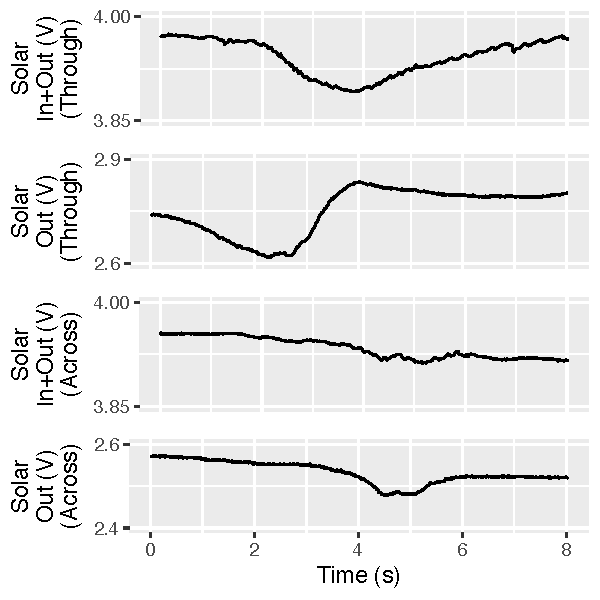
\includegraphics[width=\columnwidth]{figs/acrossAndLinger.pdf}
        \caption{ This figure compares a person walking \textit{through} the doorway (top two traces) versus walking \textit{across or by} the doorway on the outside. There is a clear delay between the two solar panel channels when someone walks through, whereas the change is reflected simultaneously when someone walks by.}
        \label{fig:across}
    \end{subfigure}
    \caption{Factors affecting \sysname operation. \label{fig:confounds}}
\end{figure*}


\paragraph{Multiple people:}
\secref{sec:normal_operation} showed the ability of \sysname to detect individual people walking through.
A practical consideration would be to consider the performance of \sysname when multiple people walk through.

In order to evaluate this, we tested two subjects walking through doorway \#1 with varying time delay between them.
This gave us control over the time separation between two events, and allowed us to examine how closely can two people walk in without being detected as one, quite large person.
We discovered that as long as two people have at least \minSeparation between them, \sysname can accurately distinguish between them.
This limitation is introduced due to the time required by the solar panels to reset or stabilize before the next event can occur.
A subsequent logical conclusion is that if two people walk side-by-side, \ie with zero separation between them, the current setup of the system is unable to detect them as two events.

\paragraph{The ``Spotlight'' effect:}
A very interesting consequence of light-based detection is what we affectionately call the \textit{spotlight effect}.
This effect appears in the presence of a very focused source of light that dominates the illumination around the doorway, such as a spotlight or a west-facing window in late evening when the sun blazes directly through.
When someone walks across such a focused light source, even if it's far from the doorway, it is detected falsely by \sysname as someone walking through.
This happens because \sysname detects people based on a decrease in the harvested energy, which also occurs when somenone momentarily blocks the focused source of light.
Interestingly, we can see from \figref{fig:spotlight} that the raw output of the solar panels look sufficiently different for someone walking \textit{across} the focused source as compared to when someone walks \textit{through} the doorway in presence of a focused source.
At present, \sysname is equipped to detect events with good accuracy.
With further signal processing, the difference between these events can be extracted so that such events will not cause false triggers.


\paragraph{Detection Range/Walking across, not through:}
\label{subsubsec:range}
Considering that \sysname uses the blocking of light to detect a person, there will be an influence radius inside which a person starts affecting the harvested energy of the sensor.
If someone walks by either side of a doorway monitored by the \sysname sensor and are within the influence radius of the sensor, they will affect the sensor readings.
We ran an experiment to determine this radius of influence where the subject was directed to walk by on either side of the doorway at increasing distances from the sensor.
We started with a distance of 1 foot and went up to 5 feet, in increments of 1 foot.
For each distance, we asked the subject to walk by multiple times and recorded how many false triggers were detected.
Our findings are presented in \figref{fig:across}.
We have observed that for distances greater than 3 feet away from the doorway, there is a negligible chance of triggering false events.

It is interesting to note from \figref{fig:across} that there is a distinguishable difference between this event as compared to someone walking through the doorway.
Since they are walking only on one side of the doorway, their effect on both channels is not delayed by the angling of the solar panels, as is the case with walking through.
As with the ``Spotlight'' effect, we should be able to extract this difference with further signal processing and learning and we attempted a stab at addressing this confounding condition further in the uncontrolled experiments that will be discussed later.  \fxnote{[This needs some serious rewording for the fact that we do try to handle this in the uncontrolled experiments.-NT]}

\paragraph{Lingering in the doorway:}
Another situation that causes false triggers is when a person comes up to the doorway, but simply pokes their head in.
Upon evaluation, we discovered that as long as the person is poking their head in the doorway, the solar panel output remains at a lower level, and when they exit, it rises back again.
Although the current system implementation isn't equipped to differentiate between someone passing through and someone lingering in doorway, there is a clear difference in the raw waveform outputted by the solar panel.
This case is similar to \secref{subsubsec:range} in terms of being distinguishable from a person walking through and with some careful, direct signal processing it is definitely possible to differentiate between the actual and the confounding case.

\subsubsection{Microbenchmarks}
\label{sec:microbenchmarks}
The more effective \sysname is at maintaining a low-power state when idling, the more available \sysname is for detecting doorway events and monitoring occupancy.
The energy requirements for detection and active computation must be kept low as well.
Unlike intermittent computing systems, \sysname must intentionally avoid power failures.
We measured the current draw of our \sysname prototype while it was mounted on doorway \#1.
The idle draw of the system was \SI{18}{\micro\ampere}, showing that \sysname can survive in a doorway with minimal light and energy harvesting.
We gathered other benchmarks of system energy performance in each mode of operation \sysname enters; the results of our experiments are shown in \tabref{tab:microbenchmarks}. These measurements were made after the MIC841 hysteresis chip, so the actual power and energy is slightly higher (by \SI{1.5}{\micro\ampere} according to the datasheet).


% Idle Current: 7-11uA, MCU not active
% Timer / ISR handling, single detector, no event : 190-230us, MCU active
% Doorway Event, MCU active, compute time: 7.2ms
%
% Peak current for active: 500uA
% Avg current for active: 220uA
% 2.8V
\begin{table*}[t]
\footnotesize
\begin{tabular}{@{}p{1.4in}lllc@{}}
\toprule
\textbf{State}          & \multicolumn{1}{r}{\textbf{Avg. Power}} & \multicolumn{1}{r}{\textbf{Peak Power}} & \multicolumn{1}{r}{\textbf{Energy Cost}} & \multicolumn{1}{r}{\textbf{MCU Active}} \\ \midrule
\textit{Waiting (Deep sleep)}       	& \SI{7}{\micro\ampere}	&  \SI{11}{\micro\ampere}	& - & \textcolor{magenta}{\xmark} \\
\textit{Maintenance Actions} & \SI{220}{\micro\ampere}	& \SI{500}{\micro\ampere}	& \SI{140}{\nano\joule}	 & \textcolor{green}{\cmark} \\
\textit{Doorway Event Handler} & \SI{220}{\micro\ampere}	& \SI{500}{\micro\ampere}	&  \SI{4424}{\nano\joule}     & \textcolor{green}{\cmark} \\ \midrule
\end{tabular}
\caption{Microbenchmarks for \sysname energy consumption.}
\label{tab:microbenchmarks}
\end{table*}


\tabref{tab:microbenchmarks} shows a low quiescent current where the MCU is asleep (the Idle state) of \SI{7}{\micro\ampere} on average. Maintenance events (from timer firing or single detectors firing from noise or people passing by the doorway but not walking through) only require \SI{140}{\nano\joule} to handle in active mode with the MCU running.
The most expensive compute operation is when the detectors fire and the MCU must compute the direction and store the results to non-volatile memory: FRAM. This costs \SI{4424}{\nano\joule}.
Overall the energy consumption of the system is low, but could be further improved with careful tuning of resistance values, sleep states, and the analog circuitry.

\begin{table*}[t]
\footnotesize
	\begin{tabular}{@{}p{0.65in}>{\centering\arraybackslash}p{0.4in}>{\centering\arraybackslash}p{0.4in}p{0.4in}p{0.5in}p{0.6in}p{0.55in}p{0.55in}p{0.55in}p{0.55in}p{0.5in}@{}}
	\toprule
	\multirow{2}{*}{\textbf{Doorway}}	&	\multicolumn{2}{c}{\textbf{Dimensions (in)}} & \multirow{2}{*}{\textbf{Light}} & \textbf{Total} & \textbf{Gnd Truth} & \textbf{Detected} & \textbf{Accounted} & \textbf{Extra} & \textbf{Missed} & \textbf{Recall}		\\
	& Height & Width &  &  \textbf{Days} & \textbf{Events} & \textbf{Events} & \textbf{Events} & \textbf{Events} & \textbf{Events}\\\midrule
	Lab & 79.5" & 34.5" & Mixed & 8 & 445 & 735 & 354 & 388 & 91 & 74.02\% \\ %Lab Door
	Hallway & 76.0" & 93.0" & Indoor & 4 & 753 & 660 & 731 & 109 & 22 & 87.66\% \\ %hallway
	Classroom & 87.0" & 35.0" & Mixed &  9 & 213 & 300 & 167 & 107 & 46 & 68.84\% \\	%232
   
	\bottomrule
	\end{tabular}
	\caption{In-the-Wild evaluation results for three different locations, from data collected over multiple days for each location. \sysname effectively detected doorway events and other activities around the sensor, while troublesome cases like people lingering under/around the sensor can produce additional event information for a single event. 
	\vspace{1mm}
	\label{tab:ITWresults}}

\end{table*}



\subsection{\sysnames in the Wild}
\begin{figure}[t]
\centering
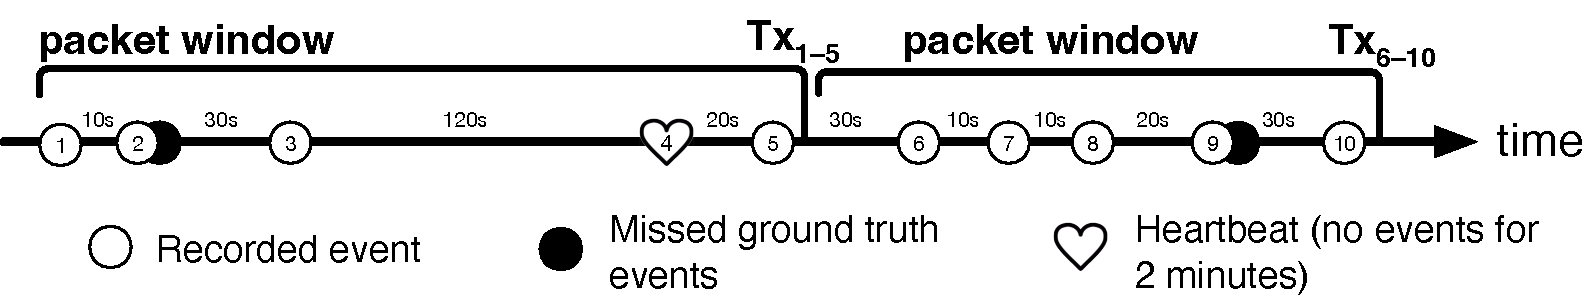
\includegraphics[width=1.0\columnwidth]{figs/timeline.pdf}
\caption{ The ground truth event timeline of our in-the-wild deployment and how it is divided up into windows based on the anchor packets.  This example provides a high level view of how we compute the event statistics within a window.  \label{fig:eventtimeline}}
\end{figure}
%setup

We conducted an extensive in-the-wild deployment of multiple \sysname units.
The controlled experiments helped us understand some of the major limits of the system, but we also wanted to see how it fared in an in-the-wild deployment.  
For a real-life application evaluation, we installed \sysname on two doorways and a hallway, gathering \ITWdays collectively of all-day occupancy data with visual (camera based) confirmation of ground truth. 

\subsubsection{In-Wild Experimental Setup.}
We chose locations---a lab door, a classroom door, and a hallway---that differ in light levels, width, and height, while providing a range of lighting and behavioral conditions. 
For example, the classroom door encounters multiple confounding cases like lingering and crowds passing under the doorway, while the lab is affected by lingering and spotlights.
Dimensions for these locations are reported in \tabref{tab:ITWresults}.  %The lab doorway is 34.5" x 79.5" and the light level is 86 lux inside the room and 91 lux outside of the room. The classroom doorway is 35" x 87" and the light level is 91 lux inside the room and 100 lux out of the room. The hallway is 76" x 93" and the light level on one side of \sysname is 94 lux and 89 lux on the other side. 
All doorways in this deployment have tile flooring and are typically well enough lit to transmit a packet once for every five detected doorway events. 
Besides \sysname devices we deployed two continuously powered basestations to collect the transmitted data from the batteryless \sysname devices.
Each basestation is an Internet-connected Raspberry Pi with a CC1101 radio that receives packets and logs them to a SQL database stored in the FLASH memory of the Pi. This data is easily retrieved for later classification of events.  

At each instrumented doorway we also place a motion activated camera that collects ground truth information by recording the actual doorway events. 
We manually labeled all recorded events by watching the videos and annotating and storing the time and a description of each event---\textit{in, out, pass-by}, as well as confounding cases like lingering and multiple people passing in or out.

We compare this source of ground truth against the events \sysname detects.
\sysname attempts to send a message to the basestation only after gathering a total of five detected events (sometimes more, since there must be enough energy to send and events may be detected while waiting for energy to send).
\sysname summarizes the events, their classifications, computes and stores a CRC over the values to protect against packet corruption and sends the summary of the collection to a nearby basestation where it will be logged for analysis. 
Each packet also encodes a small legacy of the information received in the last two packets to guard against packet loss. 

\sysname does not currently report time information, so the time the basestation receives a packet is used as a reference to match windows of events to the ground truth data.
Since \sysname reports summaries after every five events, the basestation's receive time is closely correlated to the last event in the summary.
We use these times to match likely event windows in the ground truth with received packets sent by the \sysname sensors.

%Looking at high level detection of events
\subsubsection{Data Collection and Analysis Method.}
Each packet (encodes a summary of at least 5 events) received at the basestation is matched to a likely ground truth event as long as the time between the two is less than 30 seconds.  
This helps account for human error in labeling event times as it is not always clear exactly when someone started affecting the sensor from video data.
If two events match a packet, the one closest (in time) is chosen and mapped to the 5th event associated with this packet.
Packets that map to a ground truth event are considered \textit{confirmed packets}.
All other packets that could not be mapped to an event (within 30s), are still valid packets that represent five events that \sysname detected and must be considered. 
We insert these packets into the event sequence and mark them as \textit{false positive} packets.
The false positive packets may still contain valid data associated with the ground truth.
The fifth event that generated the packet may have just been missed in the ground truth. 
These confirmed and false positive markers divide up the ground truth data into probable event windows in order to make a meaningful comparison with the packet summaries.
We then gather statistics on the number of probable events associated with each packet. 
Confirmed packets are included in the associated window counts, however, false positive packets, while still providing a meaningful anchor for the probable event window, did not have an event closely associated enough to add to the probable event window counts.  

We reason about the number of events that \sysname actually detects in these ground-truth based probable event windows by drawing on two characteristics of the system design. 
One, each packet encodes five events, and two, every packet will have a different packet id number, one greater than the last packet.
Using this knowledge, we can figure out which packets, if any, we missed (what packet id numbers were absent on the basestation?) and how well \sysname \textit{detected events}, even if it may have classified events incorrectly.
When all the ground-truth events in the event window were explained by the number of events in the anchor packet and missed packets, we considered the window to be accounted for. 
When they are not, we know that either events were recorded (on video) but not detected by \sysname, denoted as \emph{misses}, or \sysname detected more events than were reported in the ground-truth data, which we called extras. 
\figref{fig:eventtimeline} shows a high level example of the how ground truth events are divided by the anchor packet time in order to calculate extras and misses. 
These values are aggregated over all probable event windows in the ground truth data.

The results, shown in \tabref{tab:ITWresults}, are mixed.  
\sysname did a decent job of detecting when activity was taking place near the sensor, with few missed events.
After inspecting the data, nearly all misses appear to come from three situations: (1)~a person passed by the doorway, far from \sysname but still visible to the camera; (2)~multiple people passed by the door in close succession, seen as multiple events by the ground truth labelers, but only a single event by \sysname;
(3)~packets were lost due to \sysname power failures and sequences of dropped packets. 
Extra events were far higher than missed events in our data, primarily due to long and slow events---particularly common around the lab and classroom---many of which lasted minutes, were labeled as a single ground truth event but misclassified by \sysname as many events (mostly passbys).
\sysname clearly has room for improvement when classifying confounding cases like lingering and other long events and high-traffic situations; however, even in these problematic cases, \sysname serves as an effective activity sensor. \fxnote{I want to say somewhere in here that other PIR or Ultrasound-based sensors are going to have a hard time with this, too. -JMS}

%for recall event classification results
\subsubsection{Results.}
After evaluating \sysname event detection in general, we processed the data in a different way to reason about the system's classification accuracy. 
\sysname's design makes it difficult to reason about true negative events. When there was no activity, no videos were recorded and \sysname did not report events.
This is intended behavior, but without discrete negative cases statistical measures are meaningless.
Instead, we focus on the true positive rate, or Recall, as reported in \tabref{tab:ITWresults}.   

We process the data slightly differently, in order to assess how the system classified events.
We map all received packets to their closest matched ground truth event.
As before, this marks the end of the collection of ground truth events that likely contributed to the creation of the associated packet.
The matching ground truth window ends at the packet's receive time and includes up to the prior 5 events as long as they are not included in another packet's likely matched window. 
This means that some of our event windows contain fewer than five events, usually due to a linger event that is seen by \sysname as multiple events. 
We compare these likely-matched event windows to number of ins, outs, and passbys reported in the received packets and compute the true positive rate (recall).
Our classification accuracy ranged from 69-87\% depending on the location, with highest accuracy in the hallway where people tended to walk more and linger less.  


%\subsubsection{Discussion of In-Wild Results.}
%These results are impacted by people lingering by doorways, entering or exiting in crowds, making abrupt changes in direction under the sensor, and by individuals changing out cameras to collect ground truth or preforming basic system maintenance.  The matched windows to draw our comparison was impacted by sporadic camera malfunctions which limited available ground truth, collection over spring break which dampened overall user activity for several days, and a school wide power-outage for system maintenance which impacted the available light to the sensors as well as the power for the basestations to collect data and log them to the SQL database.


%\fxnote{[ I created  confusion matrix using R based on the collected data, but that data needs some cleaning like i+o, (i+)o in the %detected direction-AA]}
%section:  System Accuracy
	%just walking through
		%-just using interrupts
		%-just detection circuits
		%hw detection only vs sw enhancements
	%detecting direction
		%-just using interrupts
		%-just detection circuits
		%hw detection only vs sw enhancements
%if we get to sw at all





%section:  extreme cases (how low can we make lighting and system still work)?

\section{Related Work}
\label{sec:related}

\sysname is closely related to other occupancy-monitoring sensing systems---especially those using doorway-mounted sensor suites.
\sysname also draws from the literature on sensing systems that treat harvested energy both as energy and data signal; deriving application information from the energy source.
SolarGest~\cite{ma2019solargest} is the most recent and closely related system. SolarGest and \sysname share a similar method for using solar energy as an indicator for light ray interference, SolarGest is also batteryfree. However, SolarGest differs from \sysname in application, implementation, and focus. SolarGest measures a small set of gestures (6) that are performed close to the solar panel; these controlled conditions are in contrast to \sysname, which must deal with a wide range of confounding conditions and scenarios. Unlike SolarGest, \sysname does all recognition in-situ, while SolarGest must rely on a backscatter communication channel with which it sends all data. This offline processing severely constrains the applicability of SolarGest.


\noindpar{Occupancy-Monitoring Systems:}
Several different methods for detection of occupancy and inter-room movement have been explored. Existing occupancy monitoring systems use ultrasound\cite{hnat2012doorjamb}, imaging\cite{tyndall2016occupancy, teixeira2007lightweight}, wearables\cite{fishkin2005hands}, instrumented objects\cite{buettner2009activity}, structural vibrations\cite{pan2016occupant}, and opportunistic data leaked from existing meters and security systems\cite{yangoccupancy2014}.
These systems accurately detect occupancy (many provide other features like activity and person recognition), however, each suffers from the maintenance cost associated with battery powered systems.

AURES~\cite{shih2016aures} attempted to address this concern by using a rechargeable battery and an indoor solar panel.
AURES estimates the number of occupants in a room by using wide-band ultrasonic signals.
It needs to be installed in a central location on the room ceiling and near a light source to function properly.
AURES, as an energy-neutral system, features an extended lifetime using energy harvesting to recharge a battery.
However, all batteries wear out (usually in a few years) meaning replacement is inevitable.
In comparison, \sysname has the dual advantage of being both easy to install (on the doorway) and batteryless i.e. maintenance free.

Like AURES, EnOcean~\cite{EnOcean} and Leviton~\cite{Leviton} are commercial ceiling-mounted occupancy sensors that are also powered by harvested ambient light and utilize passive infrared sensors (PIR) for detecting occupancy through motion detection. These sensors are equipped with wireless communication capabilities for transmitting the occupancy status (occupied/not occupied) of specific rooms or areas. This is useful in controlling the lighting, HVAC and other electric loads. On the other hand, \sysname utilizes the information present in harvested energy variations to detect individual doorway movements as well as the direction of those movements. This information can not only be used in making smarter building utility decisions, it also provides a more detailed insight into area/room-wise usage of buildings in terms of occupancy count. This fine-grained occupancy information can possibly be used in optimizing the layout of a building and to provide higher flexibility in utility control.

Another work proposes a battery-free camera powered by indoor ambient light to capture and transmit images via backscatter to a basestation upon request~\cite{saffari2021battery}. Contrary to \sysname, this system uses a duty-cycle approach rather than an event-driven for detecting an occupant present, resulting in many missed events.

CeilingSee~\cite{yang2017ceilingsee} attempts to eliminate the extra power consumption of the monitoring tools by alternating existing LED lighting fixtures between being light sources and sensors in a duty cycle manner.
It uses reflected light and machine learning to distinguish between the fixed objects in the room and the rooms occupants.
CeilingSee offers a promising direction for new buildings, where custom lighting installations present an incremental cost. 
In contrast to \sysname however, applying CeilingSee to legacy installations (old buildings) would be expensive, as this would include construction costs, computational infrastructure, and IT staff maintenance.
CeilingSee could also put extra constraints on how a building can be lighted.

Recent work focuses on using multiple data sources that feed into a machine learning model to estimate the number of occupants in a building~\cite{das2017non}. Using the number of connected WiFi devices to detect occupant count can provide coarse-grained information, however it's severely limited by several possible cases such as single occupant connecting multiple devices, use of wired internet access, or not having any device connected to WiFi. This issue is addressed by monitoring utility data, such as water and electricity consumption, weather temperature, and building functions and size along with the number of WiFi devices. This combination works well at the building level. Unlike that, \sysname is designed to monitor occupancy at room-level and communicate with other similar devices to deduce building-level occupancy. 
LOCI~\cite{narayanaloci}uses data fusion from two types of sensors PIR and thermopile to localize occupants in the work space and estimates their height. It is not battryless and seems to be a power hungry system since it consume 460mW including packet transmission. 


\noindpar{Doorway Occupancy Monitoring:}
The UVa Doorjamb sensor~\cite{hnat2012doorjamb} enabled room-level tracking of people as they moved through a house, using ultrasonic range finders mounted above a doorway, pointed towards the ground. Doorjamb differentiates people by height, and detects direction of entry and exit into the doorway. 
A recent update---SonicDoor~\cite{sonicdoor-buildsys2017}---identifies occupants by sensing their body shape, movement and walking pattern using ultrasonic sensors embedded in the sides and top of the doorway. SonicDoor also senses user behaviors like wearing a backpack or holding a phone.
Doorjamb also used high-power sensors, wired power, and offline processing.
Both of systems depend on reliable power (wired power or batteries), use high-powered sensors (ultrasonic range finders), in contrast to \sysname, which uses energy harvesting and passive detection techniques to detect people walking through a doorway, providing room-level occupancy detection.

\noindpar{Energy as Data Sensing: } \sysname uses solar panels as both energy source and sensor simultaneously. This technique has been used in other systems for applications other than occupancy monitoring. Monjolo~\cite{debruin2013monjolo} measures the AC loads consumption based on the harvested power from the AC load. Trinity~\cite{xiang2013powering} is designed to measure the airflow speed of air-conditioning based on the harvested power from piezoelectricity that generated from the impact of air flow. DoubleDip~\cite{martin2012doubledip} adapted this technique to monitor the water flow through a pipe using a thermoelectric generator as a harvester and sensor. Along with these, KEH-Gait~\cite{xu2017keh} is designed for healthcare authentication and providing activity tracking. It does this by sensing the voltage level produced by two types of kinetic harvesters (piezoelectric and electromagnetic), which simultaneously also powers the system.  Similarly, SolAR~\cite{sandhu2021solar}, a wrist-worn wearable detects a variety of user activities, utilizing variation in light intensity absorbed by the solar panel as well as powering the system. There has been another attempt to design a battery-free pedometer~\cite{kalantarian2016pedometers} by placing a piezoelectric harvester inside a shoe and estimating the number of steps based on the amount of harvested energy.  

Despite the fact that there is an indoor-sensing architecture that uses indoor solar-harvested power~\cite{campbell2014energy}, this architecture does not implement the idea of using the energy harvesting source as the data sensor, as used in \sysname.
\sysname is the first batteryless energy harvesting occupancy monitoring platform, that gathers both signal as well as energy from solar panels.

\noindpar{Batteryless, Transiently Powered Sensing: }
Recent work like InK~\cite{yildirim2018ink}, HarvOS~\cite{bhatti2017harvos}, Mayfly~\cite{hester2017mayfly}, and Ratchet~\cite{van2016intermittent} have explored operating system and language-level support for developing applications easily on batteryless devices with frequent power failures.
Others have focused on energy management and storage techniques, like  Federated Energy~\cite{jhester:ufop:sensys}, to improve system uptime and responsiveness.
These systems inform our work, however, none has tackled the problem of batteryless occupancy monitoring.

\section{Discussion \& Future Work}
\label{sec:discussion}

In this paper, we demonstrated that we can monitor how people use buildings without running wires, without structural renovations, and without batteries.
Our evaluation has presented the performance of \sysname as a batteryless occupancy sensor and we also have identified corner cases that might confound the current version of the system.
This section describes our future plans in terms of making \sysname more robust and reliable.
We also present some ideas for expansion of this project.

\noindpar{Improving robustness and reliability:} \sysname in its current version depends on sudden changes in the solar panel outputs in a fairly binary manner.
It triggers when there's change and doesn't when there isn't.
This allows it to detect people walking through with high accuracy.
However, it becomes susceptible to false positives as other events might also cause a sudden change in the solar panel, for example when someone walks by the side of the door.
As discussed in \secref{sec:evaluation}, there is a visible difference between someone walking through a doorway and a false positive.
One of our goals for future work is to add direct signal processing on the microcontroller so that it will be able to access the whole shape of the waveform, and will not be reliant on the binary nature of the detector interrupts.
This will enable \sysname to be more successful in identifying people walking through the doorway with minimal false positives.

\noindpar{User perceptions of privacy:}
Occupancy monitoring is often privacy violating---cameras, audio, and other methods being examples.
Privacy rights in the workspace have long been debated~\cite{oz1999electronic}, with some workers reporting productivity suffered because of the perception of loss of privacy~\cite{stanton2000electronic}.
Even though \sysname is privacy preserving, and incapable of gathering video, audio, or other personal information, we have not yet surveyed people who live and work with \sysname in their room or office.
We believe user perceptions of their privacy could inform both the design of future \sysname prototypes and provide insight into this tension between privacy and real time occupancy monitoring.
We plan to explore this in future work.


\noindpar{Adaptability:} We plan to make the system more dynamic and flexible by providing adjustable thresholds to the detector circuit.
This will equip \sysname with the ability to tune its sensitivity to problematic cases, such as darker lighting conditions.
Another way we aim to improve the performance and adaptibility of \sysname would be to make use of learning algorithms.
Our goal is to use learning for identifying different events and separating the true positives from false ones, subsequently improving accuracy and precision.
We will introduce confidence indicators so that, even in cases where it is comparatively tougher to distinguish between those events, \sysname will be able to attach a confidence level to its prediction, broadening the range of events it can identify.
This is a feasible goal considering the evident difference between those events.

\noindpar{Network of Waldos:}
\sysname is not meant to be a standalone system in that its true potential is realized as a part of a wider network of similar sensors.
Different Waldos could exchange information to monitor occupancy on a larger scale and also to improve individual performance.
For example, if one sensor detects a large amount of traffic heading into a hallway, but none of the other sensors detect activity, it is likely that there might be some other factor that is confounding the first sensor and this knowledge could be used to refine the learning model.
Having a network of such batteryless sensors could also enable the deployment of a more sophisticated, energy-efficient communication model than simply broadcasting information opportunistically.

\noindpar{Additional sensors:} We also plan to expand the system in terms of sensing abilities by adding more sensors.
These sensors could provide various types of information such as RGB data, which could be used to semi-identify the person walking through.
This would help assign some uniqueness to each individual so that we can better track their travel through rooms in a building without gathering identifiable information that would require additional security considerations to be added to the system.
We could also opportunistically use an ultrasonic range finder in moments of high illumination to detect the height of the person passing through.

\sysname can be expanded in many different ways, as demonstrated by these ideas.


%Communication-
%currently all data is stored locally on the board and ideally we would want to be able to send the data to a basestation or central location to gain the overall benefit of making use of the room-level information that the \sysname sensor is collecting.  A network of these sensors would be necessary in a true deployment to gain a real understanding of the users and their room usage.  We are continuing to develop the system to allow for this greater flexibility and usefulness.  \fxnote{[Something like this??? -NT]}

%Alternative sensors--
%\sysname currently only uses an array of solar panels to collect energy and to gather the information necessary to determine if a person has passed through the doorway.  The system's accuracy and functionality could be improved by using additional and/or alternative sensors such as ultrasonic and RGB light sensors.  Detection is evaluated in our system only from the change in the signals that the solar panels are receiving. A change in typical color could not only be an indication of someone passing through the doorway but also a means of helping to semi-identify the person walking through.  This would help to determine some uniqueness of the individuals to better track their travel through rooms in a building without gathering identifying information that would require additional security considerations to be added to the system.  \fxnote{[Not sure which other sensors to reference-NT]}

%height estimation ---
%this can be accomplished with the ultrasonic sensors and possibly with the solar panels currently in the system alone... \fxnote{Need to elaborate with this- NT}

%adaptation --- as environments change so will energy budgets.
%We take a simple approach, that we expect to work for most indoor environments; however, within these environments there are still a great different in lighting
%We plan to explore techniques for adapting sensing modalities to match current budgets and conditions.

%recognition

%\fxnote{Not sure where to talk about it. Maybe in System Design (or here), but we should address the question about other orientations. We could put \sysname on the side of the doorway and possibly harvest more energy. Or in the floor. In the floor, it would be harder to deploy, and people would step on it, but then you break the beam directly. Lots more energy, more wear and tear, possibly more difficult signal processing from different light configurations...people we just didn't do it. Maybe we will soon.}

\section{Conclusions}
\label{sec:conclusions}

This paper has presented \sysname, a batteryless, energy-harvesting doorway-mounted sensor system for room level occupancy monitoring.
\sysname uses its energy source---generated from an array of solar cells---as data signal for detecting doorway movement, as well as the energy that powers all activities.
\sysname uses a novel, tunable, detection circuit that watches the energy harvesting signal with the processor asleep, and it is the first batteryless occupancy-monitoring system in existence.
We deployed \sysname on \numDoors doorways and found that it can detect single persons moving through the doorways with a high overall detection accuracy of \SysAccuracy. Our results show that \sysname can differentiate between entry and exit of persons walking through the doorway for \dirAccuracy of the detected events.
We also evaluated different factors that affect the performance of \sysname.
There are some events that confound the current version of \sysname into generating false positives, but we have demonstrated inherent differences from the true positives \ie someone walking through the door.
This makes us confident that we can further improve the \sysname system to make it robust to such events.
We evaluated \sysname microbenchmarks that demonstrate \sysname is low power, and efficient, able to harvest enough energy to power all activities, intermittently, while providing quality of application.
\sysname represents a first step towards robust and reliable occupancy-monitoring systems without batteries, using energy harvesting.

% ACKs only appear if anonymous flag is false for acmart.cls
\begin{acks}
This research is supported by NSF award CNS-XXXX. %1453607. 
Any opinions, findings, conclusions, and recommendations expressed in these
materials are those of the authors and do not necessarily reflect the
views of the sponsors.
\end{acks}

\balance
\bibliographystyle{ACM-Reference-Format}
\bibliography{persist}


\end{document}
